% Impostazioni principali
\documentclass[t, compress, mathserif]{beamer}



%         ----------------------------------------------         %
%        /                                              \        %
%--------               START PREAMBLE                   --------%
%        \                                              /        %
%         ----------------------------------------------         %

% Titolo che appare nella prima slide del documento
\newcommand{\titolo}{Statistics for Nominal Data}
\newcommand{\sottotitolo}{}

% Titolo che appare nella barra in basso di ogni slide, al centro
% Sono due variabili:
% * una puo' essere utilizzata per l'intero corso. Se impostata nel preambolo sovrascrive quella di seguito.
% * l'altra puo' identificare ciascun documento
\newcommand{\titolocompleto}{Statistics Course - }
\newcommand{\titoloshort}{\titolo}

% Numero di capitolo o altro nome che appare in basso di ogni slide, vicino al numero di pagina
\newcommand{\numerocapitolo}{Chapter 14}

% Include il documento che contiene il preambolo

%%%%%%%%%%%%%%%%%%%%%%%%%%%%%%%%%%%%%%%%%%%%%%%%%%%%%%%%%%%%%%%%%%%%%%%%%%%%%%
%%%%%%%%%%%%%%%%%%%%%%%%%%%% VARIABILI DA DEFINIRE %%%%%%%%%%%%%%%%%%%%%%%%%%%
%%%%%%%%%%%%%%%%%%%%%%%%%%%%%%%%%%%%%%%%%%%%%%%%%%%%%%%%%%%%%%%%%%%%%%%%%%%%%%

% Titolo che appare nella barra in basso di ogni slide, al centro
% Se impostato ha la precedenza rispetto a quello di ogni singola slide

%\renewcommand{\titolocompleto}{}

% non c'e' newcommand{\sottotitolo} perche' viene definito in ogni slide
\newcommand{\data}{}



%%%%%%%%%%%%%%%%%%%%%%%%%%%%%%%%%%%%%%%%%%%%%%%%%%%%%%%%%%%%%%%%%%%%%%%%%%%%%%
%%%%%%%%%%%%%%%%%%%%%%%%%%%%%%%%%% PACKAGES %%%%%%%%%%%%%%%%%%%%%%%%%%%%%%%%%%
%%%%%%%%%%%%%%%%%%%%%%%%%%%%%%%%%%%%%%%%%%%%%%%%%%%%%%%%%%%%%%%%%%%%%%%%%%%%%%
\usepackage[latin1]{inputenc}   
\usepackage{graphicx}
\usepackage{rotating}
\usepackage{rotfloat}
\usepackage{color}
\usepackage{colortbl}
\usepackage{../includeTex/floatflt}
\usepackage{tikz}
\usepackage{hyperref}
\usepackage{pgfpages} 
\usepackage{ifthen}
\usepackage{wasysym}
\usepackage{multirow}



%%%%%%%%%%%%%%%%%%%%%%%%%%%%%%%%%%%%%%%%%%%%%%%%%%%%%%%%%%%%%%%%%%%%%%%%%%%%%%
%%%%%%%%%%%%%%%%%%%%%%%%%%%% IMPOSTAZIONI GENERALI %%%%%%%%%%%%%%%%%%%%%%%%%%%
%%%%%%%%%%%%%%%%%%%%%%%%%%%%%%%%%%%%%%%%%%%%%%%%%%%%%%%%%%%%%%%%%%%%%%%%%%%%%%

% Beamer theme
%\usetheme{CambridgeUS}      
\usetheme{Madrid}      

% Immagini da visualizzare
\newcommand{\materiale}{minitab}

% Path delle immagini
\graphicspath{{../images/}}

% Per caricare le formule matematiche con il giusto font 
% Questo sostituisce l'opzione mathserif di documentclass (obsoleta) 
\usefonttheme[onlymath]{serif}      

     

%%%%%%%%%%%%%%%%%%%%%%%%%%%%%%%%%%%%%%%%%%%%%%%%%%%%%%%%%%%%%%%%%%%%%%%%%%%%%%
%%%%%%%%%%%%%%%%%%%%%%%%%%%%%%%%%%% COLORI %%%%%%%%%%%%%%%%%%%%%%%%%%%%%%%%%%%
%%%%%%%%%%%%%%%%%%%%%%%%%%%%%%%%%%%%%%%%%%%%%%%%%%%%%%%%%%%%%%%%%%%%%%%%%%%%%%

\definecolor{grigio}{rgb}{0.46,0.48,0.48}
\definecolor{giallo}{rgb}{1,0.84,0}
\definecolor{coolred}{rgb}{0.83,0.06,0.27}
\definecolor{arancio}{rgb}{0.97,0.46,0.09}
\definecolor{verde}{rgb}{0.25,0.78,0.25}
\definecolor{qblu}{rgb}{0.24,0.27,0.74}
\definecolor{azzurro}{rgb}{0.37,0.91,0.90}

\definecolor{grigio}{rgb}{0.46,0.48,0.48}
\definecolor{blu}{rgb}{0.25,0.28,0.78}

\definecolor{sfondoScopo}{rgb}{0.75,0.785,0.83}
\definecolor{darkred}{named}{qblu}
\definecolor{blue}{named}{qblu}

\setbeamercolor{scopo}{bg=sfondoScopo}
\setbeamercolor{section in toc}{fg=black,bg=white}
\setbeamercolor{alerted text}{fg=darkred!80!gray}
\setbeamercolor{palette primary}{fg=darkred!60!black,bg=gray!30!white}
\setbeamercolor{palette secondary}{fg=darkred!70!black,bg=gray!15!white}
\setbeamercolor{palette tertiary}{bg=darkred!80!black,fg=gray!10!white}
\setbeamercolor{palette quaternary}{fg=darkred,bg=gray!5!white}

\setbeamercolor{sidebar}{fg=darkred,bg=gray!15!white}
\setbeamercolor{palette sidebar primary}{fg=darkred!10!black}
\setbeamercolor{palette sidebar secondary}{fg=white}
\setbeamercolor{palette sidebar tertiary}{fg=darkred!50!black}
\setbeamercolor{palette sidebar quaternary}{fg=gray!10!white}

\setbeamercolor{titlelike}{parent=pallette primary,fg=darkred}
\setbeamercolor{frametitle}{bg=gray!10!white}
\setbeamercolor{frametitle right}{bg=gray!60!white}

\setbeamercolor{separation line}{}
\setbeamercolor{fine separation line}{}

%% Definizione dei colori da assegnare ai box
\setbeamercolor{postit}{fg=white,bg=qblu}
\setbeamercolor{postut}{fg=qblu,bg=gray!60!white}

%% Definizione dei colori per i diagrammi
\definecolor{bloccoIniziale}{rgb}{0.94,0.93,0.48}
\definecolor{bloccoFinale}{rgb}{0.86,0.25,0.27}
\definecolor{blocco}{rgb}{0.56,0.58,0.77}
\definecolor{bloccoSospeso}{rgb}{0.94,0.81,0.36}



%%%%%%%%%%%%%%%%%%%%%%%%%%%%%%%%%%%%%%%%%%%%%%%%%%%%%%%%%%%%%%%%%%%%%%%%%%%%%%
%%%%%%%%%%%%%%%%%%%%%%%%% STRUTTURA DELLE DIAPOSITIVE %%%%%%%%%%%%%%%%%%%%%%%%
%%%%%%%%%%%%%%%%%%%%%%%%%%%%%%%%%%%%%%%%%%%%%%%%%%%%%%%%%%%%%%%%%%%%%%%%%%%%%%

% Intestazione
\setbeamertemplate{headline}
{
  \leavevmode%
  \hbox{%
  \begin{beamercolorbox}[wd=.5\paperwidth,ht=2.25ex,dp=1ex,right]{section in head/foot}%
    \usebeamerfont{section in head/foot}\insertsectionhead\hspace*{2ex}
  \end{beamercolorbox}%
  \begin{beamercolorbox}[wd=.5\paperwidth,ht=2.25ex,dp=1ex,left]{subsection in head/foot}%
    \usebeamerfont{subsection in head/foot}\hspace*{2ex}\insertsubsectionhead
  \end{beamercolorbox}}%
  \vskip0pt%
}

% Pie' di pagina
\setbeamertemplate{footline}
{
  \hbox{%
    \begin{beamercolorbox}[wd=.20\paperwidth, ht = 2.25ex, dp = 1ex, center]{palette sidebar secondary}%
      \usebeamerfont{author in head/foot}%\insertshortauthor~~(\insertshortinstitute) 
      
\includegraphics[width=1.5cm]{QUANTIDE.jpg}
    \end{beamercolorbox}%
    \begin{beamercolorbox}[wd=.57\paperwidth, ht = 2.25ex, dp = 1ex, center]{title in head/foot}%
      \usebeamerfont{title in head/foot}{\titolocompleto \titoloshort}
    \end{beamercolorbox}%
    \begin{beamercolorbox}[wd=.13\paperwidth, ht = 2.25ex, dp = 1ex, left]{date in head/foot}%
      \hspace*{0.4em} \usebeamerfont{date in head/foot} {\numerocapitolo}
    \end{beamercolorbox}%
    \begin{beamercolorbox}[wd=.10\paperwidth, ht = 2.25ex, dp = 1ex, right]{date in head/foot}%
       \usebeamerfont{date in head/foot} \insertframenumber{} / \inserttotalframenumber \hspace*{2ex} 
    \end{beamercolorbox}%
  }%
  \vskip0pt%
}



%%%%%%%%%%%%%%%%%%%%%%%%%%%%%%%%%%%%%%%%%%%%%%%%%%%%%%%%%%%%%%%%%%%%%%%%%%%%%%
%%%%%%%%%%%%%%%%%%%%%%%%%%% STILE DELLE DIAPOSITIVE %%%%%%%%%%%%%%%%%%%%%%%%%%
%%%%%%%%%%%%%%%%%%%%%%%%%%%%%%%%%%%%%%%%%%%%%%%%%%%%%%%%%%%%%%%%%%%%%%%%%%%%%%

% Simboli di navigazione
\setbeamertemplate{navigation symbols}{}

% Modifica lo stile dell'elenco (di primo livello)
\useitemizeitemtemplate{$\star$} % Usa la stella

% Interlinea (fattore di scala; NON e' un valore assoluto)
\renewcommand{\baselinestretch}{1.2}  

% Definisci stile per vettori e matrici
\newcommand{\vect}[1]{\boldsymbol{\underline{#1}}} % Grassetto e sottolineato
\newcommand{\matr}[1]{\boldsymbol{#1}} % Grassetto

% Definire stile per valore assoluto
\providecommand{\abs}[1]{\lvert#1\rvert}
\providecommand{\norm}[1]{\lVert#1\rVert}

% Cambiare il nome delle figure e delle tabelle
\renewcommand{\figurename}{Figura}
\renewcommand{\tablename}{Tabella}

% Definizione sezioni, ecc.
\newcommand{\livelloA}{\section}
\newcommand{\livelloB}{\subsection}
\newcommand{\livelloC}{\subsubsection}

% Livello di profondita' del 'content panel' del PDF
% \hypersetup{bookmarksdepth=4} % il valore di default va bene

% Definizione prima slide
\title{\textbf{\titolo}}
\author{\sottotitolo}
\date{\data}






%         ----------------------------------------------         %
%        /                                              \        %
%--------               START DOCUMENT                   --------%
%        \                                              /        %
%         ----------------------------------------------         %

\begin{document}

% Pagina del titolo
\frame{\titlepage}

% Indice
% \section*{Table of contents}
% \begin{frame}
%   \vspace{-.5cm}
%   \footnotesize{\tableofcontents[subsectionstyle = hide/hide/hide]} 
% \end{frame}

% Documento
% I soli contenuti del documento sono in un file esterno. Questo semplifica enormemente le cose qualora si volessero creare dei manuali (singoli documenti) a partire da diversi documenti.
% \livelloA{Introduction}

% \begin{frame}
% .... da fare ....
% \end{frame}
% ======================================= %



\livelloA{Data types and random variables}

\livelloB{Data types or Data scales}
\begin{frame}
  \vspace*{.75cm}
  During the statistical analysis, data features have to be considered carefully. \\
  \vspace*{.5cm}
  The experimental phase in which information is collected is a key point: both description methods and applicable tests rely on experimental phase. \\
  \vspace*{.75cm}
  Depending on the kind of information that can be collected, \textbf{Data types} or \textbf{Data scales} can be classified into four classes.
\end{frame}

\begin{frame}
\begin{center}
\textbf{Statistical universe}
\end{center}

\vspace {0.5cm}
\onslide<1>{
\begin{tiny}
	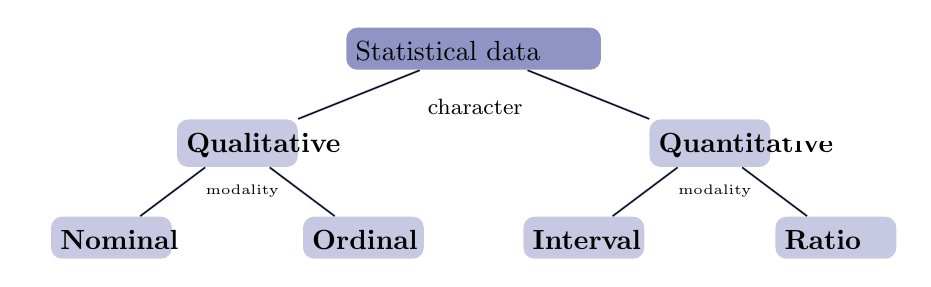
\begin{tikzpicture}[level distance=12mm] % la distanza tra i blocchi in altezza
	\tikzstyle{level 1}=[sibling distance=60mm]
                \tikzstyle{every node}=[fill=blocco!50,rounded corners,text width=1.3cm, text height=0.3cm] % la lunghezza dei blocchi
                \tikzstyle{edge from parent}=[blocco,thick,draw]
	 	\tikzstyle{level 2}=[sibling distance=32mm] % la distanza tra i blocchi in larghezza
                  \node(A1)[ text width=3cm] [fill=blocco]{Statistical data}
			child {node(B1) {\textbf{Qualitative}}
				child {node (C1) {\textbf{Nominal }}
%					child {node { \textbf{Binomial}}}
%					child {node {\textbf{Multinomial}}	}									
				}
				child {node (C2) {\textbf{Ordinal }}
				}
			}
			child {node(B2) {\textbf{Quantitative}}
				child {node  (C3) {\textbf{Interval}}}
				child {node  (C4){\textbf{Ratio}}}
			}
			
;

\path  
 (A1) 
  edge node[below=1mm,left=-23mm,fill=white]{\footnotesize character} 
 (B1);
\path  
 (A1) 
  edge node[below=3.2mm,left=-40mm,fill=white]{\footnotesize } 
 (B2);
\path  
 (B1) 
  edge node[below=-0mm,left=5mm,fill=white,text width=0.6cm, text height=0.1cm]{\tiny modality } 
 (C2);
\path  
 (B1) 
  edge node[below=-0mm,left=10mm,fill=white,text width=0.6cm, text height=0.1cm]{\tiny  } 
 (C1);

\path  
 (B2) 
  edge node[below=-0mm,left=5mm,fill=white,text width=0.6cm, text height=0.1cm]{\tiny modality } 
 (C4);
\path  
 (B2) 
  edge node[below=-0mm,left=10mm,fill=white,text width=0.6cm, text height=0.1cm]{\tiny  } 
 (C3);


         \end{tikzpicture}
\end{tiny}
}
\\
  \vspace{.35cm}
  \begin{small}
    Then, four types of scale exist: \textbf{Qualitative Nominal}, \textbf{Qualitative Ordinal}, \textbf{Quantitative Interval}, \textbf{Quantitative Ratio}\\
    \vspace{.35cm}
    This course pertains only to the analysis of \textbf{Qualitative} data.
  \end{small}
\end{frame}

\begin{frame}
  \vspace*{.15cm}
  Depending on the kind of data, different statistical options are available.\\
  \vspace*{.35cm}
  In general, on Qualitative data fewer statistical options are available than on quantitative data.\\
  \vspace*{.35cm}
  For example, on Quantitative data one might calculate the average, whereas, on qualitative nominal data this couldn't be done.\\ %% rivedere la forma dell'inglese di tutta la slide
  \vspace*{.35cm}
  Again, on Nominal data fewer statistical options are available than on Ordinal data.\\
  \vspace*{.35cm}
  Ordinal data can be treated as Nominal; the converse is not true.\\
  \vspace*{.35cm}
  Quantitative data can be always considered as Ordinal; the converse is not true.\\
\end{frame}

\livelloB{Random variables}

\begin{frame}
  A \textbf{random variable} (or \textbf{stochastic variable}) is a variable whose values are associated to a probability law. When a variable is not associated to a probability law it is called \textbf{deterministic variable}. \\
  \vspace*{.15cm}
  The \textbf{random variables} are split into two main categories that are treated in different ways:
  \vspace*{.25cm}
  \begin{enumerate}
    \item \textbf{Discrete random variables} \\
      that are usually used to model qualitative (nominal or ordinal) data frequencies.\\ 
    \item \textbf{Continuous random variables} \\
      expressed on a continuous scale of values. Values are often associated to a proper \textbf{unit of measurement}.\\
  \end{enumerate}
\end{frame}

\begin{frame}
  \vspace*{.5cm}
  The use of \textbf{discrete} or \textbf{continuous} random variables to model random phenomena is not always clearly defined, and it can depend from the number of \textbf{categories} associated to the variable.\\
%  \begin{footnotesize}
%    For example, the measurement of an height might be modeled by a discrete variable if it is measured in inches. If more decimal digits are considered then the number of categories increase and the same variable can be considered as a continuous variable.\\
%  \end{footnotesize}
  \vspace*{.75cm}
  Discrete variables have less explicative power than continuous ones:\\
 \begin{itemize}
    \vspace*{.15cm}
    \item statistics computed on continuous variables contains more information;
    \vspace*{.15cm}
    \item to get good quality statistics using discrete variables a greater \textbf{number of observations} is required.
  \end{itemize}
%During the analysis data can be split into classes. This produce more readable results at the cost of information loss. \\
\end{frame}

\begin{frame}
  \vspace*{.75cm}
  Data should be collected using the more accurate scale. When possible, data should be collected on a continuous scale. \\
  \vspace*{1cm}
  Anyway, qualitative data (or their frequencies) are almost more often modeled by discrete random variables.\\
  \vspace*{1cm}
  For the aim of this course, the data will be considered modelable as discrete random variables only. 
%More precisely, discrete random variables will model the frequency of occurrence of categories in qualitative data.
%In the case of quantitative data, the representation can be based on continuous or on discrete variables. 
%\vspace{0.5cm}
%If on qualitative data, you can define an order, take the name of ordinal modality. For example
%  \begin{footnotesize}
%\begin{itemize}
%\item Nominal data: the machine on which the measurement was taken (MO1, MO2, ...)
%\item Ordinal data: the level of goodness of the material (bad, insufficient, sufficient, good, excellent)
%\end{itemize}
%  \end{footnotesize}
%\vspace{0.5cm}
%When there are only two modality,  the data are called binomial. For example
%  \begin{footnotesize}
%\begin{itemize}
%\item Sex. The modality are: male  or female
%\item Event. The modality are: true  or false
%\end{itemize}
%  \end{footnotesize}
\end{frame}
% ======================================= %



\livelloA{Statistics for qualitative data}

\livelloB{Frequency tables}

\begin{frame}
  \vspace{0.75cm}
  Values of \textbf{frequencies} produced on the categories of a data series can be:
  \begin{itemize}
    \vspace{0.5cm}
    \item \textbf{absolute}:  the counts of observed data values in each category.
    \vspace{0.5cm}
    \item \textbf{relative}:  the  absolute frequency divided by the total count of observations
    \vspace{0.5cm}
    \item \textbf{cumulative (absolute or relative)} :  the  (absolute or relative) frequency of each category added to the sum of frequencies of lower categories. It requires ordered data.
  \end{itemize}
\end{frame}

\begin{frame}
  \vspace{0.5cm}
  The following example shows an excerpt of 50 evaluations of defective items produced by the three machines: M01, M02 e M03.\\
  \vspace*{.35cm}
  Five possibile defect levels (categories) for each article are taken: A, B, C, D and E.\\
  \vspace*{.35cm}
  The defect levels are sorted in ascending order: level A is less serious than level B, etc.. \\
  \vspace*{.35cm}
  \begin{tiny}
    \begin{center}
      \begin{tabular}{|l|c|c|c|c|c|c|c|c|c|c|c|c|c|c|c|}
        \hline      
        M01& A&B&B&D&A&A&A&E&A&D&A&B&A&....&A\\
        \hline
        M02&A&E&A&A&B&A&B&D&A&B&A&A&A&....&A\\
        \hline
        M03&A&A&D&A&B&A&A&B&A&D&A&B&A&....&B\\
        \hline
      \end{tabular}
   \end{center}
  \end{tiny}
\end{frame}

\begin{frame}
  \vspace{0.75cm}
  Considering the aggregate data on all machines, the table below reports the number of defective articles per defect type:
  \vspace{0.75cm}
  \begin{center}
    \begin{tabular}{|*{6}{c|}}
      \hline
      \textbf{Level category}  & \textbf{A} & \textbf{B} & \textbf{C} & \textbf{D} & \textbf{E} \\
      \hline
      Absolute Freq &69&43&18&9&11  \\
      \hline
      Relative Freq (\%) & 0.46 &0.29 & 0.12& 0.06& 0.07\\
      \hline
      Cumulative Abs Freq*& 69& 112 &130&139& 150\\
      \hline
      Cumulative Rel Freq *& 0.46 &0.75 & 0.87 &0.93& 1.00 \\
      \hline
    \end{tabular}\\
  \end{center}
  * only when the categories are ordered.
\end{frame}

\livelloB{Mode}

\begin{frame}
    \vspace{.35cm}
    The \textbf{mode} is the value (category) that occurs most frequently in a data series.\\
    \vspace{.35cm}
    When a phenomenon is qualitative, the value of the mode is almost the only statistics (other than frequency table) always available to summarize data.\\
    \vspace{.35cm}
    Also, the Mode is the only statistics that may be calculated either on Nominal or on Ordinal data.\\
    \vspace{.3cm}
    Frequency distributions with one mode only are called \textbf{unimodal distributions} while distributions with two or more modes are called \textbf{bimodal or multimodal distributions}.\\
    \vspace{.3cm}
\end{frame}

\livelloB{Median}
\begin{frame}
  \vspace{.75cm}
  The \textbf{median} is the category that separates the ``higher half'' of a data series from the ``lower half''. \\
  \vspace{1cm}
  It can be found by arranging all the observations from lowest value to highest value and picking the middle one.\\
  \vspace{1cm}
  For its use, at least \textbf{ordinal (or quantitative) data} are required.\\
  \vspace{1cm}
  To \textbf{calculate the median of a data series} it needs:\\
\end{frame}

\begin{frame}
  \begin{itemize}
    \item arranging all the observations from lowest value to highest value (or from the highest value to lowest value) and counting the total number $n$ of observations;
    \vspace{.15cm}
    \item if $n$ is odd, the median is the category that correnspond to the middle observation, i.e. the modality of observation in the position {\boldmath $\frac{n+1}{2}$};
    \vspace{.15cm}
    \item if $n$ is even, and the $\frac{n}{2}$-th and $\frac{n+1}{2}$-th observations belong to the same category, then this category is the median;
    \vspace{.15cm}
    \item if $n$ is even, and the $\frac{n}{2}$-th and $\frac{n+1}{2}$-th observations do not belong to the same category, then the median is undefined (or is between the two adjacent categories).
   \end{itemize}
\end{frame}

\livelloB{Mean or Average}

\begin{frame}
  \vspace{.35cm}
  When the data are of ordinal type, one might calculate the \textbf{Rank} values on data series.\\
  \vspace{.35cm}
  The ranks are numerical sequences associated to categories, such that the ordering on numerical values is the same of the ordering on categories. \\
  \vspace{.2cm}
  \begin{small}
    For example: if a \textit{Weight} ordinal character is used, with three categories (\textit{Low}, \textit{Medium}, \textit{High}), one might associate the numerical values (ranks) 1, 2, 3, respectively, to \textit{Low}, \textit{Medium}, \textit{High} categories.\\
  \end{small}
  \vspace{.35cm}
  In these cases, sometimes the average of ranks is calculated as a summary statistics.\\
  \vspace{.35cm}
  Note that this use of Average is questionable and makes sense only in specific cases.
\end{frame}

\livelloB{Contingency tables }

\begin{frame}
  \vspace{.5cm}
  \begin{columns}
    \begin{column}{0.45\textwidth}
      A \textbf{contingency table} is essentially a display format used to analyse and record the relationship between frequencies of two or more categorical variables.\\
      \vspace{.5cm}
      \begin{tabular}{|l|l|l|l|} 
        \hline
        \multirow{2}{*}{\parbox{1.5cm}{Character A}} & \multicolumn{3}{c|}{Character B}\\
        \cline{2-4}
        &B1&B2& Margin\\
        \hline
        A1 & 10\% & 1\% & 11\%\\
        A2 &  7\% & 81\% &  89\%\\
        \hline
        Margin &  17\% & 83\% & 100\%\\
        \hline
      \end{tabular}
    \end{column} 
    \begin{column}{0.4\textwidth}
      \vspace{.5cm}
      \begin{tabular}{|l|l|l|l|} 
        \hline
        \multirow{2}{*}{\parbox{1.5cm}{Character A}} & \multicolumn{3}{c|}{Character B}\\
        \cline{2-4}
        &B1&B2& Margin\\
        \hline
        A1 & 15 & 2 & 17\\
        A2 &  11 & 123 &  134\\
        \hline
        Margin &  26 & 125 & 151\\
        \hline
      \end{tabular}\\
      \vspace{.5cm}
      The contingency table, along with the frequency  table, can also be used to check if two or more phenomena can be considered independent. 
    \end{column}
  \end{columns} 
\end{frame}

\begin{frame}
  \vspace{0.5cm}
  The data of above example on Machines and Defect levels can be represented in a two-ways contingency table:
  \vspace{1cm}
  \begin{center}
    \begin{tabular}{|l|c|c|c|c|c|c|}
      \hline      
      \multirow{2}{*}{\parbox{1.5cm}{Machine}}& \multicolumn{5}{c|}{Defect level}& \\
      \cline{2-6}
      & A&B&C&D&E &Tot\\
      \hline
      M01&20&15&5&7&3&50\\	
      \hline
      M02&24&16&5&1&4&50\\
      \hline
      M03&25&12&8&1&4&50\\
      \hline
      Tot&69&43&18&9&11&150\\
      \hline
   \end{tabular}
  \end{center}
\end{frame}


\begin{frame}
  \vspace{0.5cm}
  As a table of column percents
  \vspace{1cm}
  \begin{center}
     \begin{tabular}{|l|c|c|c|c|c|c|}
      \hline      
      \multirow{2}{*}{\parbox{1.5cm}{Machine}}& \multicolumn{5}{c|}{Defect level}& \\
      \cline{2-6}
      & A&B&C&D&E &Tot\\
      \hline
      M01& 20.0\% &34.9\% &27.8\% &77.8\% &27.2\% &33.3\%\\
      \hline
      M02&34.8\% &37.2\% &27.8\%&11.1\%&36.4\%&33.3\%\\
      \hline
      M03&36.2\% &27.9\% &44.4\% &11.1\% &36.4\% &33.3\%\\
      \hline
     Tot& 100.0\% &100.0\% &100.0\% &100.0\% &100.0\% &100.0\%\\
      \hline
    \end{tabular}
  \end{center}
\end{frame}

\begin{frame}
  \vspace{0.5cm}
  As a table of row percents
  \vspace{1cm}
  \begin{center}
    \begin{tabular}{|l|c|c|c|c|c|c|}
      \hline      
      \multirow{2}{*}{\parbox{1.5cm}{Machine}}& \multicolumn{5}{c|}{Defect level}& \\
      \cline{2-6}
       & A&B&C&D&E &Tot\\
      \hline
      M01&40.0\%&30.0\%&10.0\%&14.0\%&6.0\%&100.0\%\\
      \hline
      M02&48.0\%&32.0\%&10.0\%&2.0\%&8.0\%&100.0\%\\
      \hline
      M03&50.0\%&24.0\%&16.0\%&2.0\%&8.0\%&100.0\%\\
      \hline
      Tot& 46.0\%&28.7\%&12.00\%&6.00\%&7.3\%&100.00\%\\
      \hline
    \end{tabular}
  \end{center}
\end{frame}

\begin{frame}
  \vspace{0.5cm}
  As a table of total percents
  \vspace{1cm}
  \begin{center}
    \begin{tabular}{|l|c|c|c|c|c|c|}
      \hline      
      \multirow{2}{*}{\parbox{1.5cm}{Machine}}& \multicolumn{5}{c|}{Defect level}& \\
      \cline{2-6}
      & A&B&C&D&E &Tot\\
      \hline
      M01&13.3\%& 10.0\%&3.3\%&4.7\%&2.0\%&33.3\%\\
      \hline
      M02&16.0\%&10.7\%&3.3\%&0.7\%&2.7\%&33.3\%\\
      \hline
      M03&16.7\%&8.0\%&5.3\%&0.7\%&2.7\%&33.3\%\\
      \hline
      Tot& 46.0\%&28.7\%&12.0\%&6.0\%&7.3\%&100.0\%\\
      \hline
   \end{tabular}
  \end{center}
  \vspace{1cm}
  Question: do all the tables make sense in this specific example?
\end{frame}
% ======================================= %



\livelloA{Some relevant discrete random variables}

\livelloB{Bernoulli}

\begin{frame}
  \vspace{0.35cm}
  The \textbf{Bernoulli distribution} is perhaps the simplest discrete probability distribution.\\
  \vspace{0.45cm}
  The Bernoulli distribution describes the distribution of a random phenomenon that may show only two possible outcomes (events).\\ 
  \vspace{0.45cm}
  The two events are ``labeled'' with numeric values \textbf{0} and \textbf{1}.\\
  \vspace{0.45cm}
  Usually, the event ``1'' is also named ``success''.\\
  \vspace{0.45cm}
  This distribution states that the probability of having $1$ (``success'') is $p \; (0\le p \le 1)$, and the probability of having $0$ is $1-p$.\\
\end{frame}

\begin{frame}
  \vspace{0.5cm}
  The probability function of Bernoulli distribution is then stated as:
  $$
    f(x;p)=
    \begin{cases} p & \mbox{if }x=1\\
      1-p & \mbox{if }x=0\\
      0 & \mbox{otherwise}\\
    \end{cases}
  $$\\
  \vspace{1cm}
  That can also be expressed as
  $$
    f(x;p)=p^x(1-p)^{1-x} \mbox{     for } x \in {0,1}
  $$
\end{frame}

\begin{frame}
  The Expected value (``mean'') and Variance of a Bernoulli distribution are, respectively:\\
  \vspace*{1cm}
  $E\{X\}=0\cdot(1-p)+1\cdot p=p$\\
  \vspace*{1cm}
  $ V\{X\}=E\{(X-E\{X\})^2\}=(0-p)^2 \cdot (1-p) + (1-p)^2 \cdot p=p\cdot(1-p)$
\end{frame}

\begin{frame}
  \vspace{-.2cm}
  \begin{small}
    \textbf{Example}:\\
    100 balls are contained in a bag: 
    \begin{itemize}
      \vspace{-.2cm}
      \item 80 balls are red
      \vspace{-.2cm}
      \item 20 balls are white
    \end{itemize}
    \vspace{.15cm}
    \textbf{Question:} What is the probability function about the extraction of a white ball (``success'')  from the bag in only one trial?\\
    \vspace{.3cm}
    \textbf{Answer:} Since it is known that the white balls are 20 on a total count of 100, the probability of randomly drawing 1 white ball is $p=\frac{20}{100}=0.2$, and then the probability function may be stated as:
    $$
      f(x;p=0.2)=0.2^x 0.8^{1-x} \mbox{     for } x \in {0,1}
    $$
    where $x=1$ means ``Draw a white ball'' \\ \hspace*{11cm} \Square \\
    \vspace{.3cm}
  \end{small}
\end{frame}


\begin{frame}
  \vspace{-.2cm}
  \begin{small}
    \textbf{Example}:\\
    A production machine has yielded 1300 defective units on a total of 200000 units produced in the past. \\
    \textbf{Question:} Hypothesizing that the production machine is working always in same manner, what is the probability function that describes the probability of obtaining defective/safe unit drawing randomly from the process?\\
    \vspace{.15cm}
    \textbf{Answer:} If the production process is ``stable'', we could expect that the defective rate for the machine is 1300/200000; then, the probability of having a defective unit is $p=0.0065$, and then the probability function may be stated as:
    $$
      f(x;p=0.0065)=0.0065^x 0.9935^{1-x} \mbox{     for } x \in {0,1}
    $$
    Where $x=1$ means ``Draw a defective unit'' \\ \hspace*{11cm} \Square \\
    \vspace*{.2cm}
  \end{small}
  Now, next paragraphs will show some relevant distributions that may be thought deriving from the Bernoulli distribution.
\end{frame}

% \livelloB {}
% \begin{frame}
%   There are two discrete distributions that assume significant importance for the quality in statistics\\
%   \begin{itemize}
%     \item Binomial
%     \item Poisson
%   \end{itemize}
% Both distributions explain phenomena related to the behavior of binary phenomena: false - true, defective - acceptable.\\
%   \vspace*{.2cm}
%  In particular, define the number of successes that occur in $ N $ tests given a certain probability of success of the single test.\\
%   \vspace*{.2cm}
% The two functions differ in the fact that:
%   \begin{itemize}
%     \item the Binomial studies  events with probability medium-high;
%     \item the Poisson studies  events with probability medium-low.
%   \end{itemize}
% \end{frame}
% 

\livelloB {Binomial}

\begin{frame}
  \vspace*{.3cm}
  The \textbf{binomial distribution} is the discrete probability distribution of the number of ``successes'' in a sequence of $n$ independent ``success''/``failure'' (or yes/no) experiments, each of which yields ``success'' with probability $p$.
  \vspace*{.3cm}
  $$ f(x;n,p) = \frac{n!}{x!(n-x)!}  p^x(1-p)^{n-x} \mbox{     for } x \in {0, \cdots, n}$$
  \begin{tabbing}
    where: \hspace*{.25cm} \= \\
    \hspace*{.1cm} \> $ x $ = number of successes \\
    \hspace*{.1cm} \> $ p $ = probability of success in a trial \\
    \hspace*{.1cm} \> $ n $ = number of trials \\
  \end{tabbing}
\end{frame}

\begin{frame}
  The Expected value (``mean'') and Variance of a Binomial distribution are, respectively:\\
  \vspace*{1cm}
  $E\{X\}=\displaystyle\sum_{x=0}^n x\cdot \frac{n!}{x!(n-x)!}  p^x(1-p)^{n-x}=n \cdot p$\\
  \vspace*{1cm}
  $ V\{X\}=\displaystyle\sum_{x=0}^n (x-np)^2 \cdot \frac{n!}{x!(n-x)!}  p^x(1-p)^{n-x}= n \cdot p\cdot(1-p)$
\end{frame}

\begin{frame}
  \vspace*{.5cm}
  \textbf{Example}:\\
  A coin is perfectly balanced, and we want to know the probability of having exactly 8 ``heads'' on 10 coin flips\\
  \vspace{.15cm}
  \textbf{Question:} What is the probability of having exactly 8 ``heads'' on 10 coin flips?\\
  \vspace{.25cm}
  \textbf{Answer:} Since the coin is perfectly balanced, $p=1/2$, and then the probability is:
  \vspace*{.5cm}
  $$ f(x=8;n=10,p=1/2) = \frac{10!}{8!\cdot 2!}\cdot \left(\frac{1}{2}\right) ^8 \cdot \left(\frac{1}{2}\right)^2 = 0.04 $$   \\ \hspace*{11cm} \Square \\
\end{frame}

\begin{frame}
  \textbf{Example}:\\
  A production process yields matchboxes with 100 matches each. The probability that a match does not work (defective) is 1\%. Each match is independent from the others. \\
  \textbf{Question:} What is the probability that a box contains no defective matches?\\
  \vspace{.15cm}
  \textbf{Answer:} The defective rate for the process is 1/100; then, the probability of having a defective unit is $p=0.01$, and then the probability of having 0 defectives in a box is:
  $$ f(x=0;n=100,p=0.01) = \frac{100!}{100!\cdot 0!}\cdot 0.01 ^{0} \cdot 0.99^{100} = 0.366 $$  
  \vspace*{.4cm}
  Where $x$ = \textit{Number of defective units} (or number of successes) \\ \hspace*{11cm} \Square \\
\end{frame}

\begin{frame}
  \begin{small}
    \textbf{Example}:\\
    A production process yields matchboxes with 100 matches each. The probability that a match does not work (defective) is 1\%. Each match is independent from the others. Customers require that each box contains at most 2 defective matches \\
    \textbf{Question:} Is the process compliant to customer requirements?\\
    \vspace{.15cm}
    \textbf{Answer:} The defective rate for the process is 1/100; then, the probability of having a defective unit is $p=0.01$, and then the probability of having at most 2 defective matches is:
    $$ f(x=0;n=100,p=0.01) + f(x=1;n=100,p=0.01) +  $$  
    $$ + f(x=2;n=100,p=0.01) \simeq 0.366 + 0.370 + 0.185 = 0.921$$ 
    \vspace*{.4cm}
    Where $x$ = \textit{Number of defective units} (or number of successes). \\
    Then the expected fraction of compliant boxes is about 0.921 (or 92.1\%). \\ \hspace*{11cm} \Square \\
  \end{small}
\end{frame}

\begin{frame}
  \vspace{.5cm}
  \begin {itemize}
    \item  The Bernoulli distribution is a special case of the Binomial distribution, where $n = 1$.  \\ Conversely, any binomial distribution, $B(n, p)$, is the sum of $n$ independent Bernoulli trials each with the same ``success'' probability $p$.
    \vspace{.5cm}
    \item If $p$ and  {\boldmath $ q = 1-p $}  are equal to 0.5, the distribution is always symmetrical. If $p$ is much larger or much smaller than $q$ (then $p$ and $q$ are very different), then the distribution is asymmetric. But the asymmetry decreases with the growth of $n$.
% 	\item approximations: 
% 	\begin {itemize}
% 		\item using binomial distribution when $p$ in $[0.1, 0.9]$
% 		\item using poisson distribution when $p$ not in $[0.1, 0.9]$ and $n$ isn't large
% 		\item using binomial distribution when $n$ is so large as to make {\boldmath$n \cdot p$}  is large
% 		\item using normal distribution when a sample is very large
% 	\end{itemize}
  \end{itemize}
\end{frame}

\begin{frame}
  \begin{center}
 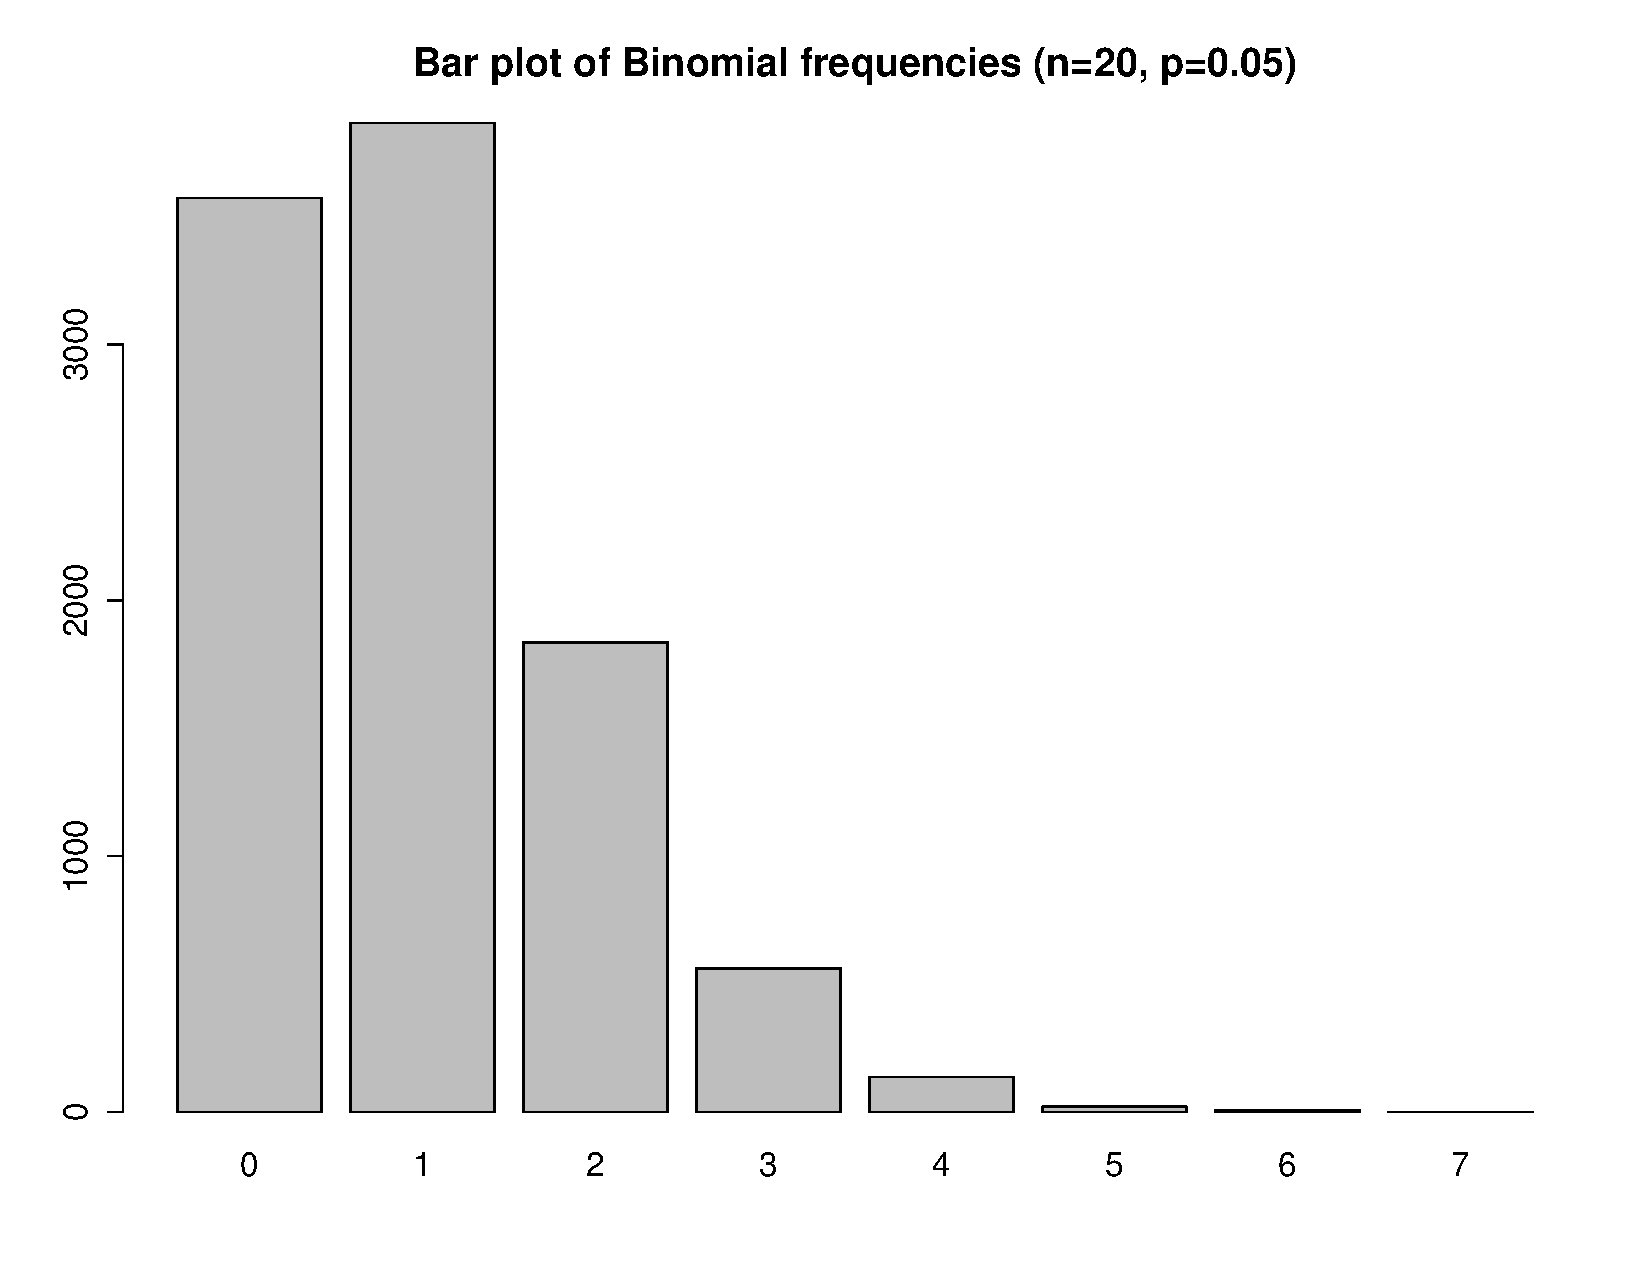
\includegraphics[width=9cm]{./../images/binomialn20p05.pdf}
 % binomialn20p05.pdf: 792x612 pixel, 72dpi, 27.94x21.59 cm, bb=0 0 792 612
\end{center}

\end{frame}

\begin{frame}
  \begin{center}
 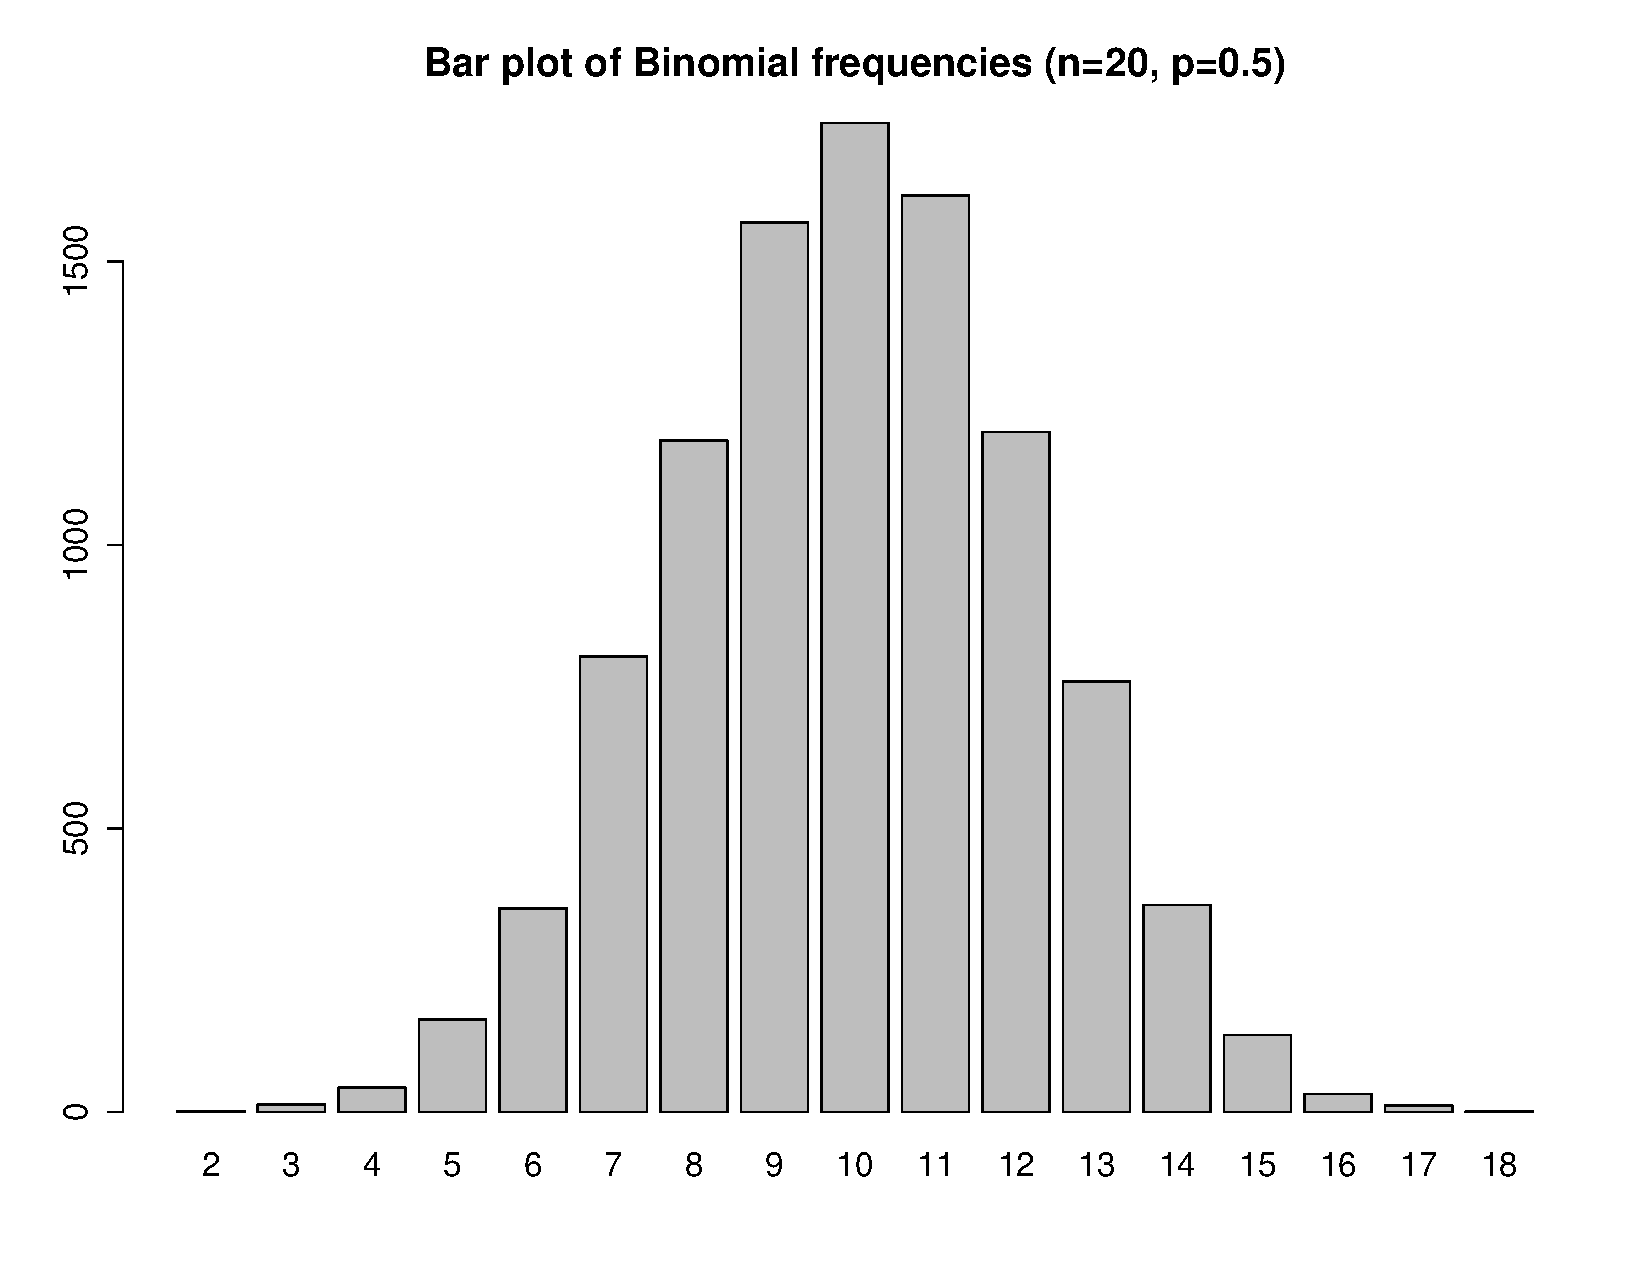
\includegraphics[width=9cm]{./../images/binomialn20p5.pdf}
 % binomialn20p05.pdf: 792x612 pixel, 72dpi, 27.94x21.59 cm, bb=0 0 792 612
\end{center}

\end{frame}

\begin{frame}
  \begin{center}
 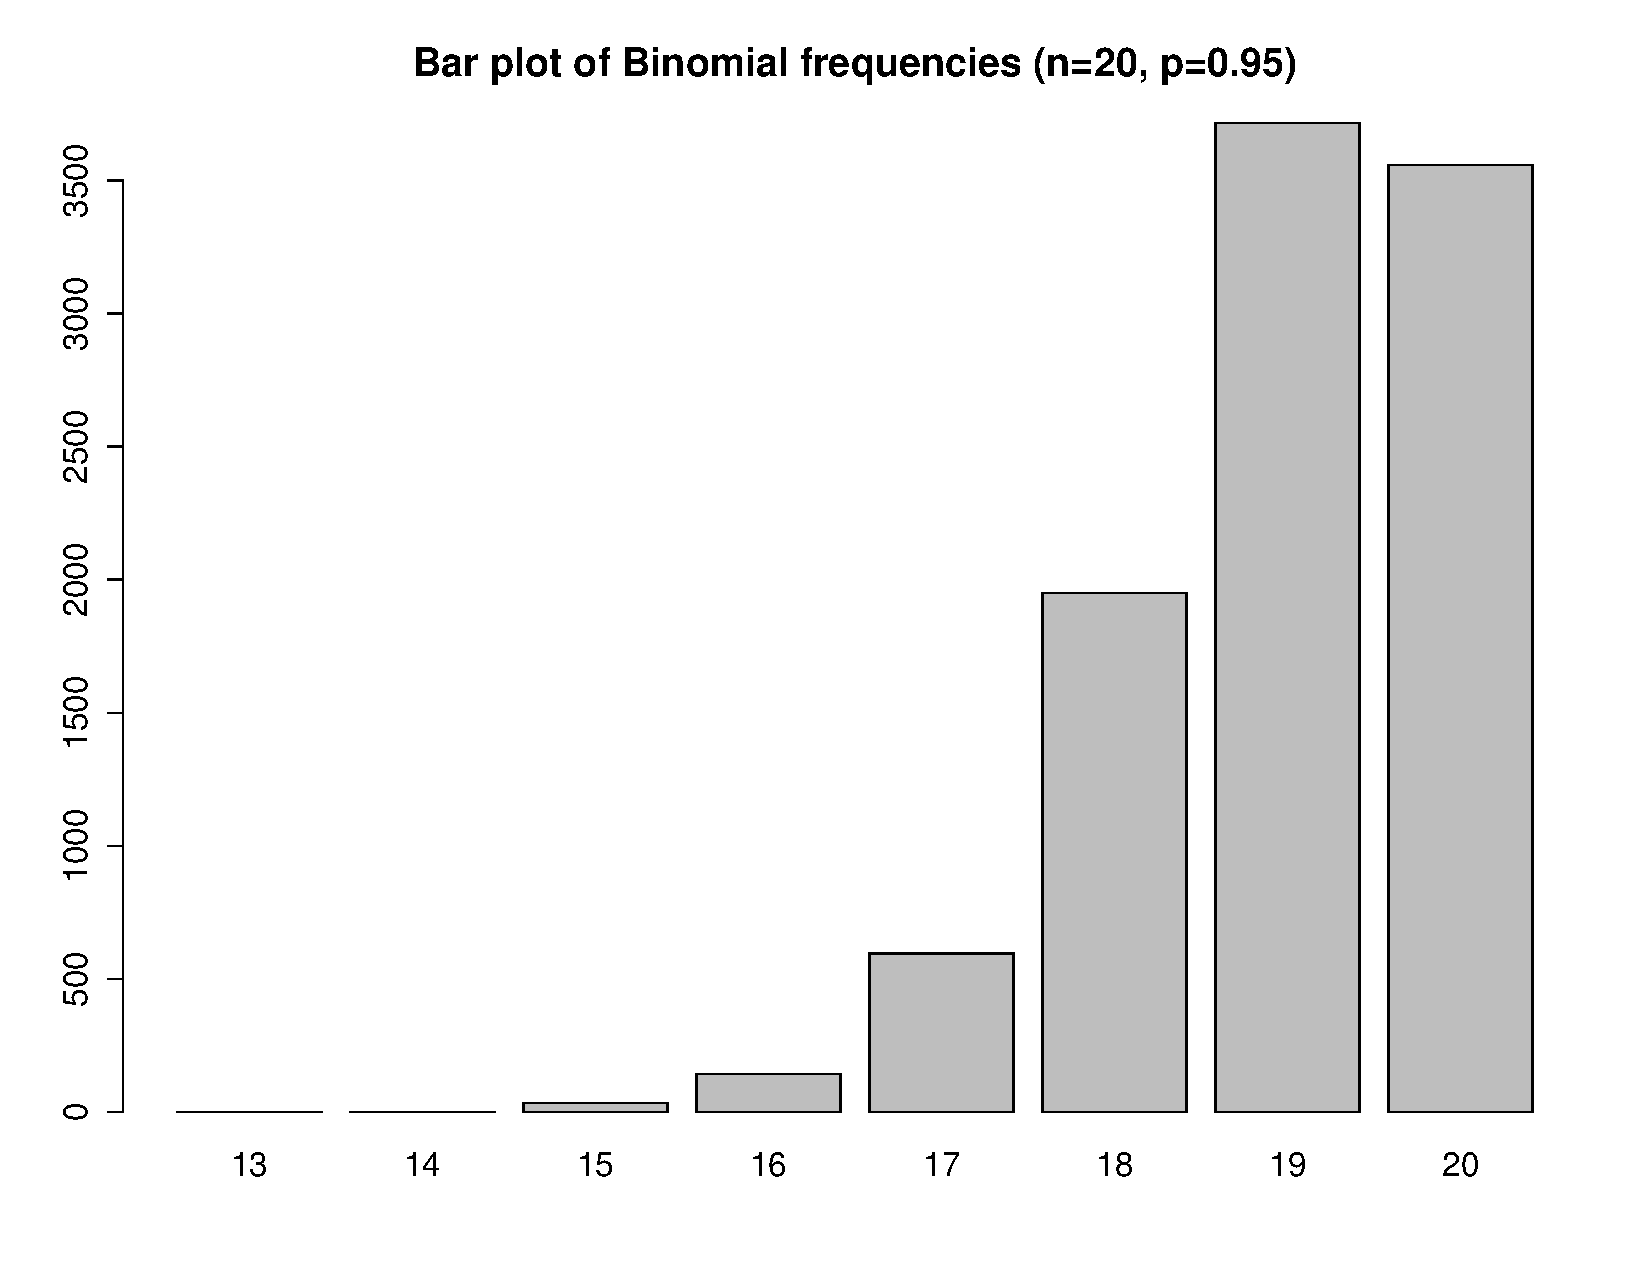
\includegraphics[width=9cm]{./../images/binomialn20p95.pdf}
 % binomialn20p05.pdf: 792x612 pixel, 72dpi, 27.94x21.59 cm, bb=0 0 792 612
\end{center}

\end{frame}

\livelloB {Poisson}

\begin{frame}
  \vspace*{.25cm}
  \textbf{The Poisson is a theoretical discrete distribution, and it is completely defined by only one parameter, {\boldmath $ \mu $}}.\\
  \vspace*{.5cm}
  The Poisson distribution is usually (but NOT always) used to  model the counts of rare random events, and its probability distribution function is:
  $$
    f(x;\mu)=\frac{\mu^x}{x!}\, e^{-\mu}  \mbox{     for } x \in {0, 1, \cdots, \infty}
  $$\\
  \vspace*{.5cm}
  The main ``conceptual'' difference between Poisson and Binomial distribution is that the count values ($x$) in Poisson distribution are virtually unlimited, whereas in Binomial distributions are limited to the number of trials ($n$).
\end{frame}

\begin{frame}
  It may be shown that the Expected value (``mean'') and Variance of a Poisson distribution are, respectively:\\
  \vspace*{1cm}
  $E\{X\}=\displaystyle\sum_{x=0}^\infty x \cdot \frac{\mu^x}{x!}\, e^{-\mu}=\mu$\\
  \vspace*{1cm}
  $ V\{X\}=\displaystyle\sum_{x=0}^\infty (x-\mu)^2 \cdot \frac{\mu^x}{x!}\, e^{-\mu}= \mu$\\
  \vspace*{1cm}
  Thus, for the Poisson distribution, expected value (mean) and variance are identical, and they equal the $\mu$ parameter.
\end{frame}

\begin{frame}
  \begin{small}
  \textbf{Example}:\\
    In a LCD display production process, the count of defects for each display is recorded. The historical average of defects counts for all the displays is 0.45. It is known that the count of defects for each display is modelable by a Poisson distribution. \\
    \textbf{Question:} What is the probability of having at most 1 defect in a randomly chosen display?\\
    \vspace{.15cm}
    \textbf{Answer:} The historical mean is 0.45, and then $\mu=0.45$. The probability of having at most 1 defect in one display, then, is:
    $$ f(x=0;\mu=0.45) + f(x=1;\mu=0.45) \simeq 0.638 + 0.287 = 0.925$$ 
    \vspace*{.4cm}
    Where $x$ = \textit{Number of defects}\\ \vspace{-.5cm} \hspace*{11cm} \Square \\
  \end{small}
  Note: $1-0.925 = 0.075$ in this case may be seen as the fraction of displays with more than one defect.
\end{frame}

\begin{frame}
  Notes:
  \begin{itemize}
    \item The Poisson distribution is a limiting case of a Binomial distribution, when $n \rightarrow \infty$, and the mean of Binomial distribution ($n\cdot p$) remains finite ($n\cdot p=\mu$). \\
    \item That's because the Poisson distribution may be used as an approximation of Binomial distribution when $p<0.05$ and $n>100$.\\
    \item The Poisson distribution may be used for events that occur either in space or in time; for example: the number of particles in a given space, or the number of arrivals in a given time span.\\
    \item Sometimes, the parameter is named $\lambda$ instead of $\mu$.\\
    \item The Poisson distribution is very (right) skewed when $\mu<1$, is still asymmetric for $\mu<3$, and is nearly symmetric and may be approximated by the normal distribution for $\mu$ greater than $6$.\\
  \end{itemize}
\end{frame}

\begin{frame}
  \vspace*{.25cm}
  This graph shows the Poisson distribution with $ \mu = 0.9$. It is right skewed.\\
  \vspace*{.5cm}
  \begin{figure}
    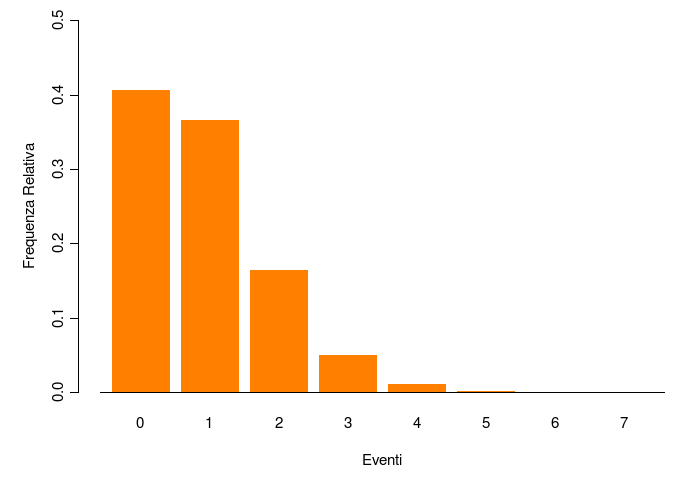
\includegraphics[scale=0.3]{2_18.png}
  \end{figure}
\end{frame}



\begin{frame}
  \vspace*{.25cm}
  This graph shows the Poisson distribution with $ \mu = 12$. It is ``almost Normal''. \\
  \vspace*{.25cm}
%   \begin{floatingfigure}[l]{6.5cm}
%     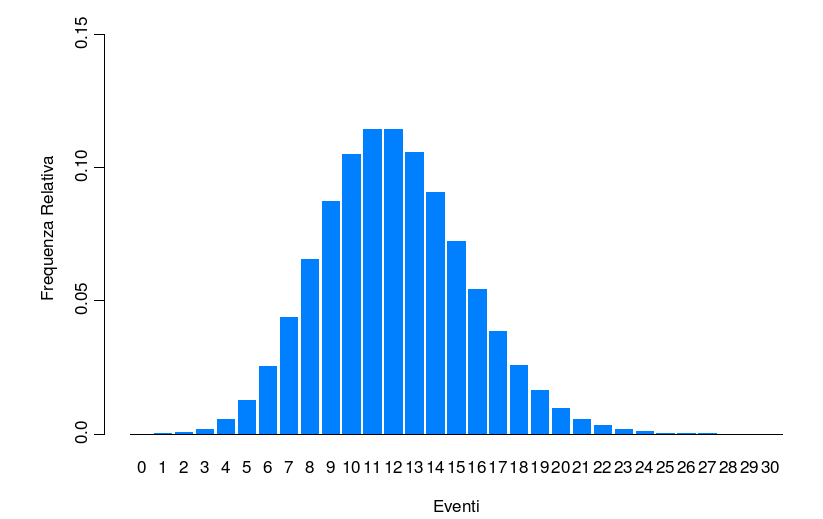
\includegraphics[scale=0.3]{2_19.png} 
%   \end{floatingfigure}
%   \hspace*{.25cm}\\
  \begin{figure}
    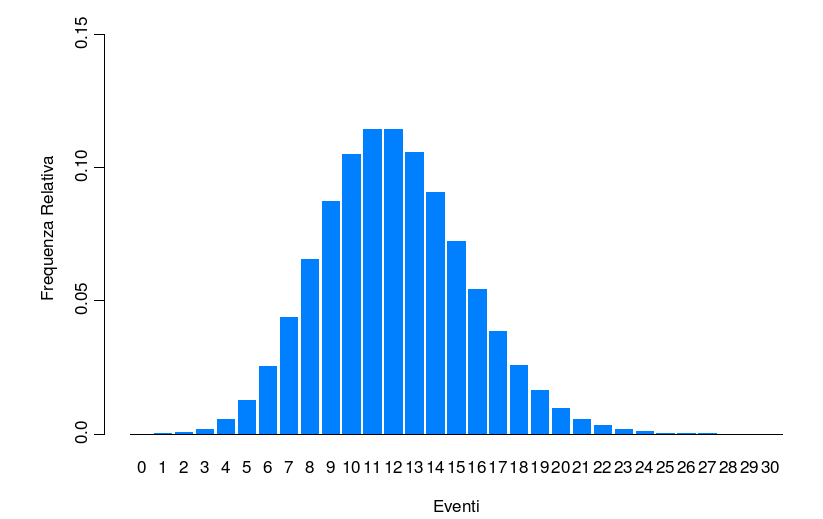
\includegraphics[scale=0.3]{2_19.png} 
  \end{figure}
\end{frame}

\livelloB {Multinomial}

\begin{frame}
  \begin{small}
    The \textbf{Multinomial} distribution is a generalization of Binomial distribution.
    The Multinomial distribution, instead of represent phenomena with only a couple of possible outcomes (TRUE/FALSE, YES/NO, ...), is used to model \textit{m}-uple of mutually exclusive categories (HIGH/MEDIUM/LOW, Green/Blue/Brown/Grey Eyes, ...). The Multinomial distribution has the following probability density function:\\
    \vspace*{.3cm}
    $$ f(x_1,...,x_m;n, p_1,...p_m)) = \frac{n!}{x_1!x_2!... x_m!} \, {p_1}^{x_1}{p_2}^{x_2}... {p_m}^{x_m} $$
    \begin{tabbing}
      where: \hspace*{.25cm} \= \\
      \hspace*{.1cm} \> $ x_i $ = number of events (``successes'') for the $i-$th ($i=1,\cdots,m$) \\
      \hspace*{2cm} category ($ x_1+x_2 + \cdots +x_m=n$ )\\
      \hspace*{.1cm} \> $ p_i $ = probability of success in only one trial for the $i-$th category \\
      \hspace*{.1cm} \> $ m $ = total number of possible categories\\
      \hspace*{.1cm} \> $ n $ = total number of trials
    \end{tabbing}
  \end{small}
\end{frame}

\begin{frame}
  \textbf{Example}:\\
  A perfectly balanced dice is thrown 8 times. \\
  \vspace{.25cm}
  \textbf{Question:} What is the probability of having 2 times ``1'', 2 times ``3'', 1 times ``4'', and 3 times ``6'' ?\\
  \vspace{.15cm}
  \textbf{Answer:} The probability may be calculated as\\
  $ f(x_1=2,x_2=0,x_3=2,x_4=1,x_5=0,x_6=3;$ \\ 
  \hspace{.3cm}$n=8, p_1=\frac{1}{6},p_2=\frac{1}{6},p_3=\frac{1}{6},p_4=\frac{1}{6},p_5=\frac{1}{6},p_6=\frac{1}{6}) = $\\
  \vspace{.3cm}
  \hspace{.3cm}$=\frac{8!}{2!0!2!1!0!3!} \, (\frac{1}{6})^{2}(\frac{1}{6})^{0}(\frac{1}{6})^{2}(\frac{1}{6})^{1}(\frac{1}{6})^{0}(\frac{1}{6})^{3}= 0.001$\\
  \hspace*{11cm} \Square \\
\end{frame}
% ======================================= %



\livelloA{Statistical inference}

\begin{frame}
  \vspace*{.75cm}
  The problem of \textbf{statistical inference} arises when the researcher obtained only a subset of overall available data (the statistical population), and he/she wants to draw decisions about the overall population. \\
  \vspace*{.75cm}
  In production set-up, these needs arise several times and in very different fields.\\
\end{frame}    

\begin{frame}
  \textbf{Example}.\\
  \begin{itemize}
    \item A factory produces switches. One researcher wants to test if the switches produced in his plant meet well some requirements on some destructive tests. The target of study is to know the fraction of switches that don't meet the requirements. Of course, in that case testing all switches is impossible.
    \vspace*{.25cm}
    \item The researcher will collect a sample of switches to assess with a given level of precision which percentage of switches will be defective in all the production process.
    \vspace*{.25cm}
    \item After that, the researcher would also test if the fraction of defective units found on the sample is compatible with the hypothesis that the true (population) percentage of defective units fall within pre-specified parameters.
  \end{itemize}
\end{frame}

\begin{frame}
  The statistical inference techniques give guidelines and formulas to obtain this kind of information.\\
  \vspace*{.25cm}
  The statistical inference techniques can be splitted in three main subgroups:
  \begin{enumerate}
    \item Point estimation techniques;
    \vspace*{.25cm}
    \item Confidence intervals evaluation;
    \vspace*{.25cm}
    \item Statistical hypothesis tests.
  \end{enumerate}
  \vspace*{.25cm}
  The techniques at the first point are usually specific of the specific problem and give intuitive enough results. The other two points are less intuitive, but they use conceptually similar techniques. 
\end{frame}
% ======================================= %



\livelloA{Point Estimation }

\begin{frame}
  The point estimation problem is usually a trivial one, when categorical data are analyzed.\\
  \vspace*{.5cm}
  Examples: 
  \begin{itemize}
    \item In a Bernoully or Binomial framework, the probability of success ($p$) may be estimated with the relative frequency of success.
    \item In case of Multinomial data, the probability of having each of the categories is estimable by the relative frequency too.
    \item In case of Poisson model, the value of $\mu$ parameter may be estimated simply with the average of counts.
  \end{itemize}
  \vspace*{.5cm}
  The problem of statistical tests and confidence interval, on the contrary, is more complex and requires more in-depth examination.
\end{frame}
% ======================================= %



\livelloA{Statistical Tests}

\begin{frame}
  Often the researcher wants to test if the analyzed phenomenon meets specific requirements.\\
  \vspace*{.5cm}
  Examples: 
  \begin{itemize}
    \item In a production process, the reasearcher could need to test if the percentage of defective units is no greater than a specific level.
    \item In medical statistics, one might want to test if the fraction of medical patients that heal after the use of a drug is equal to some percentage.
    \item In banking industry, one may want to check if two groups of customers have the same level of bankrupt percentage.
  \end{itemize}
  \vspace*{.5cm}
  The researcher often can draw only a sub-sample of the overall population, and he/she have to draw conclusions about the overall population.
\end{frame}

\begin{frame}
  \vspace*{.3cm}
  All the above example assertions could be stated in mathematical form, and they are examples of so-called \textbf{Null hypoteses} (\boldmath$H_0$).\\
  \vspace*{.3cm}
  The null hypothesis is the main hypothesis stated by the researcher about a phenomenon to be tested.\\
  \vspace*{.3cm}
  To conduct a statistical test, the Null hypothesis must be tested against an alternative hypothesis.\\
  \vspace*{.3cm}
  The alternative hypothesis is usually called $H_1$ or $H_A$. \\
  \vspace*{.3cm}
  $H_0$ and $H_A$ must be mutually exclusive and exhaustive.\\
  \vspace*{.3cm}
  Statistical tests give methods and criteria to assess if $H_0$ or $H_A$ is true, based on sample data, with a pre-assigned error probability.\\
\end{frame}

\livelloB{1 Proportion Test}

\begin{frame}
  Suppose that a sample of $n$ observations from the population has been drawn to test the ``success'' probability.\\
  \vspace*{.3cm}
  If the number of observed ``successes'' is denoted with $x$, and each sample unit has a ``success'' (e.g., percentage of defective units) probability $p$ and it is independent from the others, then, prior to sample extraction, $x$ will be a Binomial random variable, with parameters $n$ and $p$. \\
  \vspace*{.3cm}
  The researcher could want to test the hypothesis that the true (and unknown) proportion $p$ of ``successes'' is equal to $ p_0 $. \\
  This is the null hypothesis, and it is stated as:
  \boldmath$H_0: p=p_0$\\
  \vspace*{.5cm}
  The alternative hypothesis $H_A$ could be that the true (population) proportion $p$ of ``successes'' is different from $p_0$. In mathematical form:
  \boldmath$H_A: p\neq p_0$
\end{frame}

\begin{frame}
  This results to an \textbf{hypothesis system}:
  \vspace{-0.25cm} 
  \begin{tabbing}
    \=  $ H_0 $ \= $ :  p = p_0 $,\\
    \>  $ H_A $ \> $ :  p \neq p_0 $.\\
  \end{tabbing}
  \vspace{-0.75cm} 
  Denoting with the symbol $ \hat{p} = \frac{x}{n} $ the observed proportion of ``successes'' within the sample, the simplest \textbf{test statistics} that allow to test $H_0$ against $H_A$ is the following:
  $$ \frac{\hat{p} - p_0}{\sqrt{p_0 (1-p_0) / n}} $$
  If $H_0$ is true, and $n$ is sufficently large, then the above quantity (prior conducting the sample extraction) will be distributed as a standard Normal distribution.\\
  If $H_A$ is true, and $n$ is sufficently large, then the above quantity will be distributed as a normal distribution centered ``away from zero''.
\end{frame}

\begin{frame}
 \begin{itemize}
  \vspace{0.5cm}
  \item If $H_0$ is true, then one expects that the value of above formula, after the experiment, will lie between the values -1.96 and 1.96 with probability $0.95 (=1-\alpha)$.
  \vspace{0.5cm}
  \item If, conversely, $H_A$ is true, then one expects that the value of above formula, after the experiment, will lie away from 0.
  \vspace{0.5cm}
  \item Then, a couple of thresholds could be selected, at -1.96 and 1.96: 
  \begin{itemize}
    \item if the value of test statistics falls between these limits, then $H_0$ is accepted (or, equivalently, $H_A$ is rejected); 
    \item if the value of test statistics falls outside these limits, then $H_0$ is rejected (or, equivalently, $H_A$ is accepted).
  \end{itemize}
 \end{itemize}
\end{frame}


\begin{frame}
  \begin{figure}
    \centering
    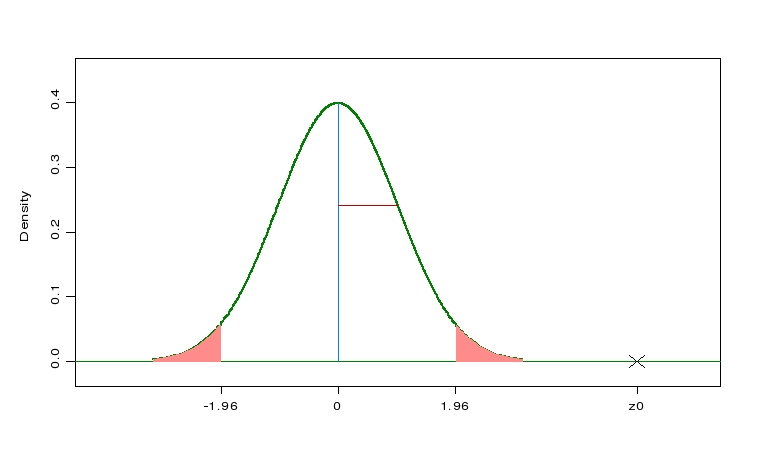
\includegraphics[width=10.5cm]{3_16.png}
    % ZtestBi.png: 800x800 pixel, 72dpi, 28.22x28.22 cm, bb=0 0 800 800
  \end{figure}
  Reject the Null hypothesis ($H_0$), and accept $H_A$.
\end{frame}


\begin{frame}
  \begin{figure}
    \centering
    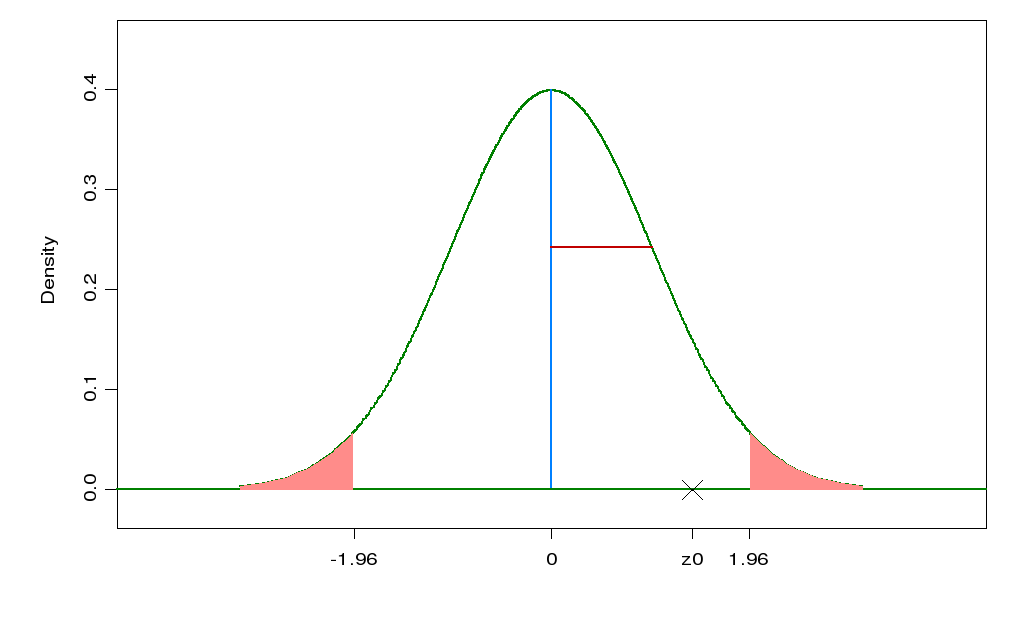
\includegraphics[width=10.5cm]{3_17.png}
    % ZtestBi.png: 800x800 pixel, 72dpi, 28.22x28.22 cm, bb=0 0 800 800
  \end{figure}
  Accept the Null hypothesis ($H_0$), and reject $H_A$.
\end{frame}

\begin{frame}
  \textbf{IMPORTANT NOTES:} 
  \begin{itemize}
    \item Given the above thresholds, $H_0$ may be erroneously rejected, when $H_0$ is true, with probability 0.05.
    \vspace{0.15cm}
    \item Changing the threshold values, the probability ($\alpha$) of erroneously rejecting $H_0$ changes too.
    \vspace{0.15cm}
    \item The $\alpha$ value (0.05 in above example) is called \textbf{significancy level}.
    \vspace{0.15cm}
    \item The $1-\alpha$ value (0.95 in above example) is called \textbf{confidence level}.
    \vspace{0.15cm}
    \item The test presented is said a \textbf{two-sided test}, because $H_A$ states that $p$ is different from $p_0$. If $H_A$ states that $p$ is strictly greater (or less) than $p_0$, the test is said \textbf{one-sided test}, and the threshold to accept/reject $H_0$ changes, to obtain the same $\alpha$ level.
  \end{itemize}
\end{frame}

\begin{frame}
  \textbf{Example}.\\
  \vspace{0.25cm}
  The management of a DVD manifacture company needs to test the hypothesis that the fraction of defectives units in the process is 0.01 (=1\%). \\
  The significancy level at which the test is performed is $ \alpha = 0.05 $.\\
  \vspace{0.25cm}
  With that aim, a sample of 100 units is randomly drawn from the process. After functional tests, only two units appear defective.\\
  \vspace{0.25cm}
  To check the null hypothesis $ H_0: p = 0.01 $ against the alternative hypothesis $ H_A: p \neq 0.01 $ the above test statistics is used:
  $$ \frac{(2/100) - 0.01}{\sqrt{0.01 (1-0.01) / 100}} = 0.01 / \sqrt{0.000099} = 1.005 $$\
\end{frame}

\begin{frame}
  \vspace{0.25cm}
  Since the absolute value of 1.005 is less than the threshold value 1.96, then one can say that \textbf{there's no empirical evidence to reject the null hypothesis}.\\ 
  \vspace{0.5cm}
  \textbf{The same conclusion may be drawn by reading the p-value}: the probability (calculated on the standard Normal distribution) of having a value of test statistics outside the interval given by -1.005 and 1.005.\\
  This probability is 0.315.\\
  Since the p-value is greater than the chosen $ \alpha $ value, the null hypothesis is accepted.\\
  \vspace{0.25cm}
  \textbf{IMPORTANT NOTE}: the p-value is the usual manner of reading tests results.
\end{frame}

\begin{frame}
%  \vspace{0.25cm}
  An $(1-\alpha)$ \textbf{confidence interval} for the ``true'' fraction of ``successes'' may be generated, following the same guidelines used for the statistical test. The confidence interval is given by:
  $$ \left( \hat{p} - z_{1-\frac{\alpha}{2}} \cdot \sqrt{\frac{\hat{p} (1-\hat{p})}{n}}; \hat{p} + z_{1-\frac{\alpha}{2}} \cdot \sqrt{\frac{\hat{p} (1-\hat{p})}{n}} \right) $$\\
  If $\alpha=0.05$, then $z_{1-\frac{\alpha}{2}}=1.96$.\\
  \textbf{Example (continue)}.\\
  The ``true'' fraction of defective DVDs, at a $ 0.95 $ confidence level, with the above example data, is:
  $$ \left( \frac{2}{100} - 1.96 \cdot \sqrt{\frac{0.02 (1-0.02)}{100}}; \frac{2}{100} + 1.96 \cdot \sqrt{\frac{0.02 (1-0.02)}{100}} \right) $$\\
  \vspace{-0.15cm}
  i.e., the interval $ \left(-0.0074; 0.0474\right) $.
\end{frame}

\begin{frame}
  \textbf{IMPORTANT NOTES:}
  \begin{itemize}
    \item The methods shown to construct statistical tests or confidence intervals for one proportion are the simplest ones, and rely on asymptotic behavior of statistcal test when $n$ is ``big''.\\
    \item An exact version of statistical test and a better approximation of confidence intervals are available.
    \item The $\alpha$ value is a conventional one. A different value of $\alpha$ may be chosen, with different error probabilities. The most used $\alpha$ values are 0.1, 0.05, 0.01, 0.001, with the second and third ones more frequently used.
    \item Confidence interval and statistical test usually give the same information: if the test accepts $H_0$, the confidence interval ``encloses'' the hypothesized value $p_0$, and viceversa.
  \end{itemize}
\end{frame}

\livelloB{2 Proportions Test}

\begin{frame}
  If one wants to compare the fraction of ``successes'' ($ p_A $ and $ p_B $) between two independent sub-populations starting from some sample data, the statistical test that he/she should use is the 2 Proportions Test.\\
  The general form of 2 proportion test null hypothesis states that the difference of proportion of ``successes'' in two sub-populations are equal to a given value $\delta_0$. The hypothesis system, then, may be stated as:\\
  \vspace{-0.15cm}
  \begin{tabbing}
    \=  $ H_0 $ \= $ :  p_A - p_B = \delta_0$\\
    \>  $ H_A $ \> $ :  p_A - p_B \neq \delta_0$\\
  \end{tabbing}
  \vspace{-1cm}
  And in its simplest form, the 2 proportions test is:
  $$ \frac{(\hat{p}_A - \hat{p}_B)-\delta_0}{\sqrt{\hat{p}_A (1 - \hat{p}_A) / n_A + \hat{p}_B (1 - \hat{p}_B) / n_B}} $$\\
  \vspace{-0.15cm}
  If $ H_0 $ is true, and for $ n_A $ and $ n_B $ large enough, the distribution of test statistics is approximately a standard Normal.
\end{frame}

\begin{frame}
  \vspace{0.25cm}
  \textbf{Example}:\\
  Suppose that two production machines, A and B, produced, in one working day, respectively 200 and 500 units. Among the units, 3 units of machine A and 4 units of machine B were flawed.\\
  \vspace{0.25cm}
  \textbf{Question}: Do the two machines produces the same proportion of defective units ($H_0: \delta_0=0$), or the two machines produce different proportions of defective units ($H_A:\delta_0 \neq 0$)? The requested error probability is $\alpha = 0.05 $.\\
  \vspace{0.25cm}
  \textbf{Answer}:
  By using the above formula, the results are:
  $$ \frac{(3/200) - (4/500)}{\sqrt{(3/200) (1 - (3/200)) / 200 + (4/500) (1 - (4/500)) / 500}} = 0.73 $$
\end{frame}

\begin{frame}
  \vspace{0.25cm}
  Since the absolute value of above quantity (0.73) is less than the threshold value of a standard normal distribution for $ \alpha = 0.05 $, (1.96), then one may state that \textbf{there's no empirical evidence that allows to reject the Null hypothesis}.\\
  \vspace{0.5cm}
  The same conclusions may be drawn by reading the p-value (the probability of having a value ``external'' to the values -0.73 and 0.73 on a standard normal distribution). This probability is 0.465.\\
  Since the p-value is greater than the fixed $ \alpha $ value, the null hypothesis is accepted.
\end{frame}

\begin{frame}
  \vspace{0.5cm}
  \textbf{NOTES:}\\
  \vspace{0.75cm}
  \begin{itemize}
    \item Several ``forms'' of two proportions test statistics are available; the proposed form is conceptually the simplest.\\
    \vspace{0.75cm}
    \item As for the one proportion test, for the two proportions test the one-sided alternative hypothesis is available. The threshold value, and the p-value, can be obtained in a similar manner than for one proportion test.
  \end{itemize}
\end{frame}

\livelloB{Chi-square Observed Vs Expected}

\begin{frame}
  \vspace{0.25cm}
  The preceding tests may be applied when the analyzed phenomenon has a Bernoulli or a Binomial distribution, or when the researcher is mostly interested to one specific category of analyzed dimension.\\
  \vspace{0.35cm}
  When the phenomenon can produce more than two outcome categories, and the researcher is interested in all (or more than only one) categories, then the one-proportion or the two-proportions test may be inadequate.\\
  \vspace{0.35cm}
  Suppose that the observed phenomenon may assume $m$ distinct values (categories), and that the researcher needs to test, based on a observation sample, if the $m$ individual categories have a ``success'' probability equal to specific values $p_{1_0}, \cdots, p_{m_0}$, where $\sum_{1=1}^m p_{i_0}=1$.\\
  \vspace{0.25cm}
  This is a case of Multinomial distribution
\end{frame}


\begin{frame}
  \vspace{0.25cm}
  The hypothesis test system, then, may be stated as:\\
  \vspace{0.25cm}
  $H_0: p_1=p_{1_0}, \cdots, p_m=p_{m_0}$\\
  $H_A: \exists i \mbox{ } (i \in 1, \cdots, m) \mbox{ }  | \mbox{ }  p_i \neq p_{i_0}$\\
  \vspace{0.75cm}
  In other words:
  \begin{itemize}
    \item $H_0$ states that the probability of success of each category is equal to its pre-specified value;
    \vspace{0.25cm}
  \item $H_A$ states that the probability of success for at least one category is different from its pre-specified value.
  \end{itemize}
\end{frame}


\begin{frame}
  \vspace{0.25cm}
  To test this hypothesis system, given a sample of $n$ independent observations, one must:
  \begin{itemize}
    \vspace{0.25cm}
    \item Calculate the frequency table for the observed phenomenon, obtaining the \textbf{Observed frequency counts} $O_1, \cdots O_m$
    \vspace{0.35cm}
    \item Calculate the \textbf{Expected frequency values} as $E_1=n \cdot p_{1_0}, \cdots , E_m=n \cdot p_{m_0}$
    \vspace{0.35cm}
    \item Calculate the following (Pearson) \textbf{Chi-square statistics}:  \\
    $$\chi^2=\sum_{i=1}^m\dfrac{(O_i-E_i)^2}{E_i}$$
  \end{itemize}
\end{frame}

\begin{frame}
  \vspace{0.25cm}
  If $H_0$ is true, then one expects (prior the experiment) that the $\chi^2$ statistics tends to be distributed (as $n$ increases) as a well-known $\chi_{m-1}^2$ distribution, and that its value will be relatively small.\\
  \vspace{0.25cm}
  If $H_0$ is false (and then $H_A$ is true), then one expects (prior the experiment) that the $\chi^2$ statistics \textbf{shall not} be distributed as a $\chi_{m-1}^2$ distribution, and that its value will be relatively large.\\
  \vspace{0.25cm}
  An upper threshold on the $\chi_{m-1}^2$ distribution may then be chosen so that the probability of obtaining a $\chi^2$ test value greater or equal than the threshold is $\alpha$.\\
  \vspace{0.25cm}
  Alternatively, one may calculate the probability on the $\chi_{m-1}^2$ distribution to give a value greater or equal than the observed  $\chi^2$ test value, obtaining the  p-value.
\end{frame}

\begin{frame}
  \vspace{0.5cm}
  If, after the experiment, the observed $\chi^2$ value is greater than the threshold value, or (equivalently) if the calculated p-value is less than the pre-assigned $\alpha$ level, then one must reject the null hypothesis ($H_0$), and accept the alternative hypotesis ($H_A$).\\
  \vspace{0.75cm}
  If, on the contrary, the observed $\chi^2$ value is less than the threshold value, or (equivalently) if the calculated p-value is greater than the pre-assigned $\alpha$ level, then one must accept the null hypothesis ($H_0$), and reject the alternative hypotesis ($H_A$).
\end{frame}

\begin{frame}
  \textbf{Example:}
  Suppose, in the above example on defects per machine, that the researcher expects that the incidence of defects follows the percentages:\\
  \vspace{0.25cm}
  $H_0: p_{A_0}=50\%, p_{B_0}=25\%, p_{C_0}=12\%, p_{D_0}=8\%, p_{E_0}=5\% $.\\
  \vspace{0.25cm}
  The researcher needs to test (at a $\alpha=0.05$ level) if the above sample confirm this rule or, conversely, if the sample pushes to reject this hypothesis. The observed table of defects frequency counts is:\\
  \vspace{0.25cm}
  \begin{center}
    \begin{tabular}{|c|c|c|c|c|c|}
      \hline      
       A&B&C&D&E &Tot\\
      \hline
     69&43&18&9&11&150\\
\hline
 \end{tabular}
\end{center}
  \vspace{0.25cm}
In this example, $m$=5.
\end{frame}

\begin{frame}
  \textbf{Example (continued):}
  The expected frequencies, based on expected percentages are:\\
  \vspace{0.25cm}
  \begin{center}
    \begin{tabular}{|c|c|c|c|c|c|}
      \hline      
      A&B&C&D&E &Tot\\
      \hline
      75&37.5&18&12&7.5&150\\
      \hline
    \end{tabular}
  \end{center}
  \vspace{0.35cm}
  The calculation of $\chi^2$ test statistics gives:\\
  $$\chi^2=\frac{(69-75)^2}{75}+ \frac{(43-37.5)^2}{37.5}+\cdots + \frac{(11-7.5)^2}{7.5}\simeq 3.67$$\\
  \vspace{0.35cm}
  If $H_0$ is true, this quantity should come from a $\chi^2_{m-1}=\chi^2_{4}$ distribution.
\end{frame}

\begin{frame}
  \textbf{Example (continued):}\\
  \vspace{0.25cm}
  \begin{figure}[h!]
   \centering
   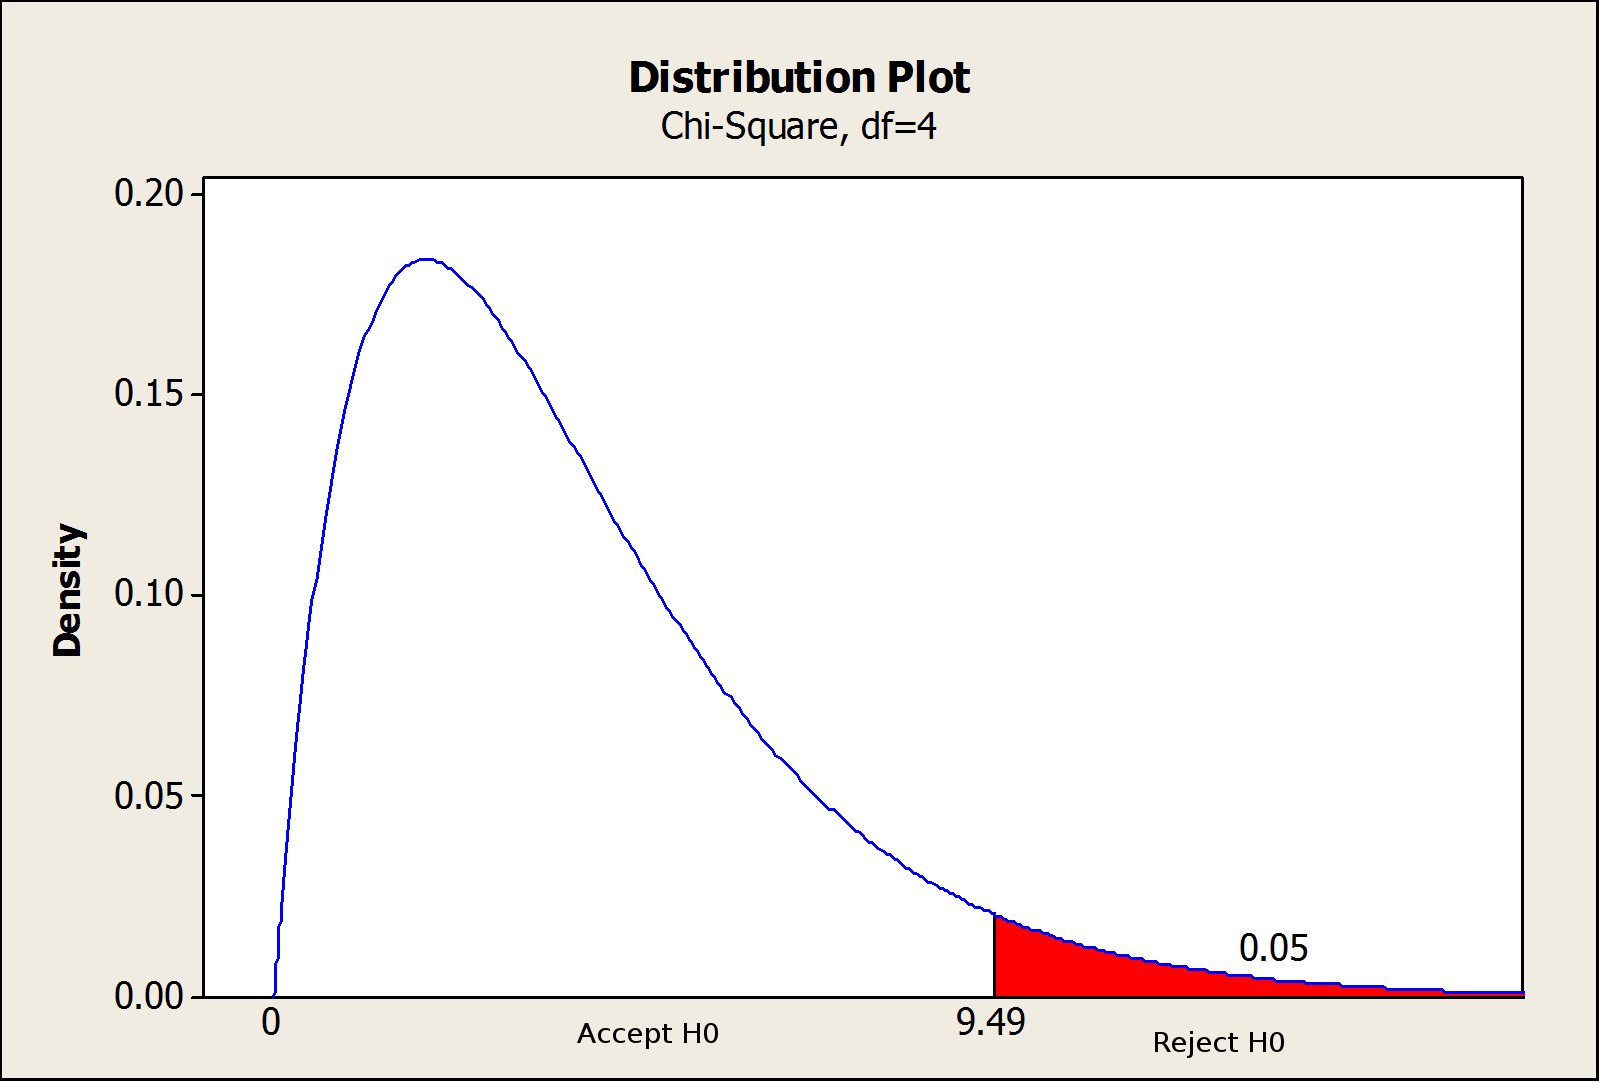
\includegraphics[width=10cm]{chi2dist.png}
   % chi2dist.png: 1600x1082 pixel, 200dpi, 20.32x13.74 cm, bb=0 0 576 390
  \end{figure}
\end{frame}

\begin{frame}
  \textbf{Example (continued):}\\
  \vspace{0.35cm}
  Since the threshold to accept/reject $H_0$ for a $\chi^2_4$ distribution is 9.49, and the test statistic is less than this threshold, the researcher must accept the $H_0$ hypothesis.\\
  \vspace{0.35cm}
  In other words, \textbf{there is no evidence in data to reject the null hypothesis} and to accept the alternative hypotesis.\\
  \vspace{0.35cm}
  Alternatively, the researcher could calculate the p-value, i.e., the probability on a $\chi^2_4$ distribution of having values greater or equal to the obtained statistics (=3.67). \\
  \vspace{0.35cm}
  In this case, the p-value is 0.453, greater than $\alpha$ (=0.05).  \\ \hspace*{11cm} \Square \\
\end{frame}

\begin{frame}
  \textbf{IMPORTANT NOTES:}\\
  \begin{itemize}
  \item The Chi-square Observed Vs Expected is an asymptotic test; that means that it needs sufficiently large sample sizes ($n$: total number of units tested) to be applicable.\\
  \item The expected cell count (i.e., the expected number of events for the individual categories) is also expected being greater than 5 to obtain ``good'' asymptotic results.
  \item When the sample size is too small, the test tends to be less ``precise'', i.e., it tends to reject or accept the null hypothesis with greater probability than expected.\\
  \item See also the indications for the test of next paragraph.
  \item \textbf{DO NOT confuse the $\chi^2$ test statistics with the $\chi^2$ distribution!}
  \end{itemize}
\end{frame}

\livelloB{Chi-square for Contingency tables}

\begin{frame}
  \vspace*{.25cm}
  This test may be seen as an ``extension'' of preceding two tests.\\
  \vspace*{.25cm}
  It tests \textbf{if the categories of two qualitative dimensions measured on the same units are associated or not}.\\
  \vspace*{.25cm}
  To exemplify this test, a simplification of above example on production machines is used.\\
  \vspace*{.25cm}
  Suppose then that a sample of $n$ units coming from 3 production machines (A, B, C) has been tested to check for the presence of defective units. The researcher needs to check if the number of (or the percentage of) defective changes with the production machine.\\
  \vspace*{.25cm}
  In other words, the researcher needs to test if there is an association between production Machine and Defects.
\end{frame}

\begin{frame}
  \vspace*{.5cm}
  Suppose that a sample of 430 units were drawn from production process, and that the data were summarized as in table below.\\
  \begin{table}
    \begin{tabular}{|c|c|r|r|}
      \cline{3-4}
      \multicolumn{2}{c}{} & \multicolumn{2}{|c|}{Units state}\\ \cline{3-4}
      \multicolumn{2}{c}{} & \multicolumn{1}{|c|}{\hspace*{.25cm}Safe\hspace*{.25cm}} & \multicolumn{1}{|c|}{Defective}\\ \hline
      & \multicolumn{1}{|c|}{\hspace*{.5cm}A\hspace*{.5cm}} & \multicolumn{1}{|r|}{132} & \multicolumn{1}{|r|}{13}\\ \cline{2-4}
      \multicolumn{1}{|c|}{Machine} & \multicolumn{1}{|c|}{B} & \multicolumn{1}{|r|}{99} & \multicolumn{1}{|r|}{18}\\ \cline{2-4}
      & \multicolumn{1}{|c|}{C} & \multicolumn{1}{|r|}{157} & \multicolumn{1}{|r|}{11}\\ \hline
    \end{tabular}
  \end{table} 
  \vspace*{.5cm}
  The table can be represented in percentage form, and then two alternative (but equivalent) hypotheses on these percentages could be made
\end{frame}

\begin{frame}
  \begin{footnotesize}
    Each machine has the same percentage of defective units.\\
  \end{footnotesize}
  \begin{table}
    \begin{tabular}{|c|c|r|r|}
      \cline{3-4}
       \multicolumn{2}{c}{} & \multicolumn{2}{|c|}{Units state}\\ \cline{3-4}
      \multicolumn{2}{c}{} & \multicolumn{1}{|c|}{\hspace*{.25cm}Safe\hspace*{.25cm}} & \multicolumn{1}{|c|}{Defective}\\ \hline
      & \multicolumn{1}{|c|}{\hspace*{.5cm}A\hspace*{.5cm}} & \multicolumn{1}{|r|}{91.0\%} & \multicolumn{1}{|r|}{9\%}\\ \cline{2-4}
      \multicolumn{1}{|c|}{Machine} & \multicolumn{1}{|c|}{B} & \multicolumn{1}{|r|}{84.6\%} & \multicolumn{1}{|r|}{15.4\%}\\ \cline{2-4}
      & \multicolumn{1}{|c|}{C} & \multicolumn{1}{|r|}{93.5\%} & \multicolumn{1}{|r|}{6.5\%}\\ \hline
    \end{tabular}
  \end{table} 
  \vspace*{.5cm}
  \begin{footnotesize}
    The percentage of machines within defective units and within safe units is constant.
  \end{footnotesize}
  \begin{table}
    \begin{tabular}{|c|c|r|r|}
      \cline{3-4}
      \multicolumn{2}{c}{} & \multicolumn{2}{|c|}{Units state}\\ \cline{3-4}
      \multicolumn{2}{c}{} & \multicolumn{1}{|c|}{\hspace*{.25cm}Safe\hspace*{.25cm}} & \multicolumn{1}{|c|}{Defective}\\ \hline
      & \multicolumn{1}{|c|}{\hspace*{.5cm}A\hspace*{.5cm}} & \multicolumn{1}{|r|}{34.0\%} & \multicolumn{1}{|r|}{31.0\%}\\ \cline{2-4}
      \multicolumn{1}{|c|}{Machine} & \multicolumn{1}{|c|}{B} & \multicolumn{1}{|r|}{25.5\%} & \multicolumn{1}{|r|}{42.9\%}\\ \cline{2-4}
      & \multicolumn{1}{|c|}{C} & \multicolumn{1}{|r|}{40.5\%} & \multicolumn{1}{|r|}{26.2\%}\\ \hline
    \end{tabular}
  \end{table} 
  \vspace*{.5cm}
\end{frame}

\begin{frame}
  \vspace*{.25cm}
  Each of two above statements can be equivalently expressed as:\\
  \vspace*{.25cm}
  $ H_0 $: No association exists between Machines and Defectives.\\
  \vspace*{.25cm}
  Against the alternative hypothesis:\\
  \vspace*{.25cm}
  $ H_A $: An association exists between Machines and Defectives (or, ``The defective percentage is different for at least one machine'' or ``At least one machine has a percentage within defective units and within safe units different from the others'').\\
  \vspace*{.25cm}
  \textbf{NOTE:} If no association exists between Machine and Defectives, then one expects that the within row percentages (and within columns percentages) are constant and equal to the columns marginal percentages (and row marginal percentages).
\end{frame}

\begin{frame}
  In more general form: suppose that two qualitative characteristics where read on  $n$ sampled units. The first characteristic (Q1) has $r$ categories, while the second one (Q2) has $c$ categories. The researcher needs to test if the distribution of two characteristics \textbf{is not associated} within the overall population.\\
  The following contingency table may be built:\\
  \begin{table}
    \begin{tabular}{|c|c|c|c|c|}
      \hline
      \multicolumn{1}{|c|}{} & \multicolumn{3}{|c|}{Q2} & \multicolumn{1}{|c|}{}\\ \hline
      & $n_{11}$ & $\cdots$ & $n_{1c}$ & $n_{1.}$ \\ \cline{2-5}
      Q1  & $\cdots$ & $n_{ij}$ & $\cdots$ & $\cdots$ \\ \cline{2-5} 
      & $n_{r1}$ & $\cdots$ & $n_{rc}$ & $n_{r.}$ \\ \hline
      & $n_{.1}$ & $\cdots$ & $n_{.c}$ & $n$ \\ \hline
    \end{tabular}
  \end{table}
  \vspace{-0.15cm}
  where $ n_{ij} $ is the number of units with $ i $-th category of Q1 and $ j $-th category of Q2; $ n_{i.} $ is the $ i $-th row total, and $ n_{.j} $ is the $ j $-th column total.
\end{frame}

\begin{frame}
  \vspace*{.25cm}
  If we denote with $ p_{ij} $ the relative frequencies within columns $ (p_{ij} = n_{ij}/n_{.j}) $, then, if no association exists between characteristics, one expects that: $ p_{i1} = p_ {i2} = \dots = p_{ic} = p_{i.} $, $ (i = 1, \, \dots, \, r) $, where $ p_{i.} = n_{i.}/n $\\
  \vspace*{.25cm}
  In other words, the relative frequencies calculated within the columns are all equal, and are equal to the marginal relative frequencies. \\
  \vspace*{.5cm}
  The same sentence may be stated by calculating the relative frequencies within the rows: $ p_{1j} = p_{2j} = \dots = p_{rj} = p_{.c} $, $(j = 1, \, \dots, \, c) $, where $ p_{.j} = n_{.j}/n $\\
  \vspace*{.5cm}
  As stated above, the two forms are ``equivalent''.
\end{frame}

\begin{frame}
  \vspace*{.05cm}
  Taking the first of two forms, if absolutely no association exists between the two qualitative characteristics, then one expects that:\\
  \vspace*{-.3cm}
  $$ p_{ij}=p_{i.} \Longleftrightarrow n_{ij}/n_{.j} = n_{i.}/n  \Longleftrightarrow n_{ij} = (n_{i.} \cdot n_{.j})/n $$\\
  \vspace*{.1cm}
  The last equality is the mathematical condition because no association exists between the two characteristics.\\
  Then, given a two-way contingency table, the above formula allows to assess what shall be the frequencies values within the cells if ``perfect independence'' (i.e. loss of association) exists between the two characteristics: $ n_{ij}^* \, ( = (n_{i.} \cdot n_{.j})/n) $\\
  The (Pearson) \textbf{Chi-square test}, then, uses the following formula to test if no association exists:
  $$ \chi^2 = \sum_{i=1}^r \sum_{j=1}^c{\frac{(n_{ij}-n_{ij}^*)^2}{n_{ij}^*}} $$
\end{frame}

\begin{frame}
  \vspace{0.25cm}
  If $H_0$ is true, then one expects (prior the experiment) that the $\chi^2$ statistics tends to be distributed (as $n$ increases) as a $\chi_{(c-1)\cdot(r-1)}^2$ distribution, and that its value will be relatively small.\\
  \vspace{0.25cm}
  If $H_0$ is false (and then $H_A$ is true), then one expects (prior the experiment) that the $\chi^2$ statistics \textbf{shall not} be distributed as a $\chi_{(c-1)\cdot(r-1)}^2$ distribution, and that its value will be relatively large.\\
  \vspace{0.25cm}
  An upper threshold on the $\chi_{(c-1)\cdot(r-1)}^2$ distribution may then be chosen so that the probability of obtaining a $\chi^2$ test value greater or equal than the threshold is $\alpha$.\\
  \vspace{0.25cm}
  Alternatively, one may calculate the probability on the $\chi_{(c-1)\cdot(r-1)}^2$ distribution to give a value greater or equal than the observed  $\chi^2$ test value, obtaining the p-value.
\end{frame}

\begin{frame}
  \vspace{0.75cm}
  If, after the experiment, the observed $\chi^2$ value is greater than the threshold value, or (equivalently) if the calculated p-value is less than the pre-assigned $\alpha$ level, then one must reject the null hypothesis ($H_0$), and accept the alternative hypotesis ($H_A$).\\
  \vspace{1cm}
  If, on the contrary, the observed $\chi^2$ value is less than the threshold value, or (equivalently) if the calculated p-value is greater than the pre-assigned $\alpha$ level, then one must accept the null hypothesis ($H_0$), and reject the alternative hypotesis ($H_A$)
\end{frame}


\begin{frame}
    \textbf{NOTES:}
    \begin{itemize}
      \vspace{0.5cm}
      \item The above result is asymptotic; this means that it needs large sample sizes ($ n>100 $).
      \vspace{0.5cm}
      \item Particularly, statistics literature suggests to not having expected frequency counts ($ n_{ij}^* $) less than 5.\\
      \vspace{0.5cm}
      \item Some authors say that at most 2 or 3 cells are allowed with expected count less than 5.
    \end{itemize}
\end{frame}

\begin{frame}
  \begin{footnotesize}
    Let's come back to the above example. The observed counts are:\\
    \vspace*{.2cm}
    \hspace*{2cm}
    \begin{tabular}{|c|c|r|r|r|}
      \cline{3-4}
      \multicolumn{2}{c}{} & \multicolumn{2}{|c|}{Units state} & \multicolumn{1}{c}{}\\ \cline{3-5}
      \multicolumn{2}{c}{} & \multicolumn{1}{|c|}{\hspace*{.25cm}Safe\hspace*{.25cm}} & \multicolumn{1}{|c|}{Defective} & \multicolumn{1}{c|}{\hspace*{.25cm}Tot \hspace*{.25cm}}\\ \hline
      & \multicolumn{1}{|c|}{\hspace*{.5cm}A\hspace*{.5cm}} & \multicolumn{1}{|r|}{132} & \multicolumn{1}{|r|}{13} & \multicolumn{1}{|r|}{145}\\ \cline{2-5}
      \multicolumn{1}{|c|}{Machine} & \multicolumn{1}{|c|}{B} & \multicolumn{1}{|r|}{99} & \multicolumn{1}{|r|}{18} & \multicolumn{1}{|r|}{117}\\ \cline{2-5}
      & \multicolumn{1}{|c|}{C} & \multicolumn{1}{|r|}{157} & \multicolumn{1}{|r|}{11} & \multicolumn{1}{|r|}{168}\\ \hline
      \multicolumn{1}{c}{} & \multicolumn{1}{|c|}{Tot} & \multicolumn{1}{|r|}{388} & \multicolumn{1}{|r|}{42} & \multicolumn{1}{|r|}{430}\\ \cline{2-5}
    \end{tabular}\\
    \vspace*{.4cm}
    While the expected counts are:\\
    \vspace*{.2cm}
    \hspace*{2cm}
    \begin{tabular}{|c|c|r|r|}
      \cline{3-4}
      \multicolumn{2}{c}{} & \multicolumn{2}{|c|}{Units state}\\ \cline{3-4}
      \multicolumn{2}{c}{} & \multicolumn{1}{|c|}{\hspace*{.25cm}Safe\hspace*{.25cm}} & \multicolumn{1}{|c|}{Defective}\\ \hline
      & \multicolumn{1}{|c|}{\hspace*{.5cm}A\hspace*{.5cm}} & \multicolumn{1}{|r|}{130.84} & \multicolumn{1}{|r|}{14.16}\\ \cline{2-4}
      \multicolumn{1}{|c|}{Machine} & \multicolumn{1}{|c|}{B} & \multicolumn{1}{|r|}{105.57} & \multicolumn{1}{|r|}{11.43}\\ \cline{2-4}
      & \multicolumn{1}{|c|}{C} & \multicolumn{1}{|r|}{151.59} & \multicolumn{1}{|r|}{16.41}\\ \hline
    \end{tabular}\\
    \vspace*{.5cm}
    The test statistic value: 6.271 \hspace*{1cm} $Pr\{\chi_2^2>6.271\}=0.043$
  \end{footnotesize}
\end{frame}

\livelloB{Fisher exact test for 2x2 tables}

\begin{frame}
  \vspace*{.25cm}
  When the sample size ($n$) is small, or when many expected cell counts are less than 5, the Chi-square test statistics may produce unreliable results.\\
  \vspace*{.75cm}
  Some literature suggests to use the so-called Yate's correction, which reduces the absolute value of each difference between observed and expected frequencies by 0.5 before squaring.\\
  \vspace*{.75cm}
  But its use is a matter of discussion between statisticians.\\
  \vspace*{.75cm}
  When the the contingency table is a 2x2 table, then an exact Chi-square test is available: the Fisher Chi-square test.
\end{frame}


\begin{frame}
  \vspace*{.25cm}
  Suppose to have a 2 by 2 contingency table as the following:\\
  \vspace*{.25cm}
  \begin{table}
    \begin{tabular}{|c|c|r|r|}
      \cline{3-4}
      \multicolumn{2}{c}{} & \multicolumn{2}{|c|}{Units state}\\ \cline{3-4}
      \multicolumn{2}{c}{} & \multicolumn{1}{|c|}{\hspace*{.25cm}Safe\hspace*{.25cm}} & \multicolumn{1}{|c|}{Defective}\\ \hline
      & \multicolumn{1}{|c|}{\hspace*{.5cm}A\hspace*{.5cm}} & \multicolumn{1}{|r|}{$a$} & \multicolumn{1}{|r|}{$b$}\\ \cline{2-4}
      \multicolumn{1}{|c|}{Machine} & \multicolumn{1}{|c|}{B} & \multicolumn{1}{|r|}{$c$} & \multicolumn{1}{|r|}{$d$}\\ 
    \hline
    \end{tabular}
  \end{table} 
  \vspace{.25cm}
  Where $a, b, c, d$ are cell counts, and $a + b + c + d=n$.\\
  \vspace{.25cm}
  Fisher showed that the probability of obtaining any such set of values, given marginal counts, is given by:
  $$\dfrac{(a+b)!(c+d)!(a+d)!(b+d)!}{a!b!c!d!n!}$$
\end{frame}


\begin{frame}
  \vspace*{.25cm}
  In order to test if association \textbf{does not exist} ($H_0$) between the two characteristics, the total probability of observing data `as extreme' or more extreme when the null hypothesis is true must be calculated.\\
 \vspace{.25cm}
  The above probability for all these tables must be calculated, and add them together. \\
 \vspace{.25cm}
  This gives a one-tailed test. \\
 \vspace{.25cm}
  For a two-tailed test we must also consider tables that are equally extreme but in the opposite direction. \\
 \vspace{.25cm}
  Unfortunately, classification of the tables according to whether or not they are `as extreme' is problematic, but almost all the software packages give an option to calculate these values, and then the Fisher test.\\
\end{frame}

\livelloB{Proportions tests and Chi-square test}

\begin{frame}
  \vspace{.5cm}
  When the comparison of proportions with some reference values, or when two proportions should be compared, then the 1 proportion or the 2 proportions test (respectively) can be applied.\\
  \vspace{.75cm}
  The above $\chi^2$ tests might be seen as an alternative or a generalization of 1 proportion or 2 proportions tests, with two-sided alternative hypothesis .\\
  \vspace{.75cm}
  Consider, for example, the 1 proportion test example:\\
  $H_0: p=0.01$\\
  $H_A: p\neq 0.01$\\
  \vspace{.25cm}
\end{frame}

\begin{frame}
  \vspace{.25cm}
  The above test may be ``translated'' in a ``Chi-square Observed Vs Expected'' problem, rewriting it in following contingency table:
  \vspace{.25cm}
  \begin{center}
  \begin{tabular}{l|c|c}
  & $O_i$ & $E_i$\\
  \hline
  Defective & 2 & 1\\
  Safe & 98 & 99\\
  \hline
  \end{tabular}
  \end{center}
  \vspace{.25cm}
  In that case, the Chi-square test gives:\\
  \vspace{.25cm}
  $$\chi^2=\dfrac{(2-1)^2}{1}+\dfrac{(98-99)^2}{99}\simeq 1.01010$$\\
  \vspace{.25cm}
  With a p-value, calculated on a $\chi^2_1$ distribution, of $0.315 > 0.05 (=\alpha)$, very close to the above (1 proportion) result.
\end{frame}

\begin{frame}
  \vspace{.25cm}
  If we consider the 2 proportions test example, the test is:\\
  $H_0: p_A=p_B$\\
  $H_A: p_A\neq p_B$\\
  \vspace{.25cm}
  If the sample data are rewritten in tabular form:
  \begin{center}
  \begin{tabular}{l|c|c}
  & Machine A & Machine B\\
  \hline
  Flawed & 3 & 4\\
  Safe & 197 & 496\\
  \hline
  \end{tabular}
  \end{center}
  \vspace{.25cm}
  $$\chi^2=\dfrac{(3-2)^2}{2}+\dfrac{(4-5)^2}{5}+\dfrac{(197-198)^2}{198}+\dfrac{(496-495)^2}{495}\simeq 0.707$$\\
  With a p-value, calculated on a $\chi^2_1$ distribution, of $0.400 > 0.05 (=\alpha)$, close to the above (2 proportions) result.
\end{frame}


\begin{frame}
  \vspace{.25cm}
  \textbf{NOTES:}\\
  \vspace{.25cm}
  \begin{itemize}
   \item Chi-square tests may be seen as alternative tests to 1 proportion or 2 proportions tests.
   \item Chi-square tests may be used only when the alternative hypotesis is two-sided.
   \item Chi-square tests can manage also more than one or two proportions only; in that sense they are a generalization of ``x proportions'' tests.
   \item In cases when the sample size is small, and the asymptotic approximation could not be applied, then the Yate's correction or (when possible) the Fisher exact test can be used. In above example, the Fisher exact test gives a p-value of $0.4140$, very close to the above p-values.
  \end{itemize}


\end{frame}

% % ======================================= %
% \livelloA{Relative Risk Ratios for 2x2 table, and Odds-ratio}
% % ======================================= %
% \begin{frame}
% .... da fare ....
% \end{frame}

\livelloB{Mantel-Haenszel-Cochran Chi-square}

\begin{frame}
  \vspace{.25cm}
  Let's take again the last example, and suppose in this case that three samples were drawn: one sample for each of three raw material suppliers.\\
  \vspace{.25cm}
  The aim of the test is always to check if \textbf{there's no association} between production Machine and Defectives:\\
  \vspace{.25cm}
  $H_0$: No association exists between Machine and Flaws presence.\\
  $H_A$: Some association exists between Machine and Flaws presence.\\
  \vspace{.25cm}
  Since the three suppliers can produce materials with different quality levels, the researcher expects that aggregating all the sample data in only one sample, without considering differences between suppliers, could bias the results.
\end{frame}

\begin{frame}
  \vspace{.25cm}
  In this case, the hypothesis system must be rewritten in this form:\\
  \vspace{.25cm}
  \begin{description}
   \item[$H_0$:] No association exists between Machines and Flaws presence within categories of Suppliers.
   \item[$H_A$:] Some association exists between Machines and Flaws presence within categories of Suppliers.\\
   \end{description}
  \vspace{.25cm}
  The \textbf{Mantel-Haenszel-Cochran Chi-square test} allows to test this type of hypothesis system for a set of $k$ 2 by 2 contingency tables.\\
  \vspace{.25cm}
  In this example, $k=3$ is the number of suppliers, and the 2x2 tables are the individual ``Machines Vs Defectives'' contingency tables.
\end{frame}

\begin{frame}
  \vspace{.5cm}
  If the four numbers in 2 by 2 tables are labeled like this:\\
  \begin{center}
    \begin{tabular}{cc}
      $a_j$ & $b_j$\\
      $c_j$ & $d_j$\\
    \end{tabular}
  \end{center}
  \vspace{.25cm}
  where $j=1, \cdots, k$, and $(a_j+b_j+c_j+d_j)=n_j$, the equation for the Mantel-Haenszel-Cochran test statistic may be written as\\
  $$\chi^2_{MHC}=\dfrac{\left(\left|\sum_{j=1}^k a_j-(a_j+b_j)(a_j+c_j)/n_j\right|-0.5\right)^2}{\sum_{j=1}^k (a_j+b_j)(a_j+c_j)(b_j+d_j)(c_j+d_j)/(n_j^3-n_j^2)}$$
\end{frame}

\begin{frame}
  \vspace{0.25cm}
  If $H_0$ is true, then one expects (prior the experiment) that the $\chi^2_{MHC}$ statistics tends to be distributed as a $\chi_1^2$ distribution, and that its value will be relatively small.\\
  \vspace{0.25cm}
  If $H_0$ is false (and then $H_A$ is true), then one expects (prior the experiment) that the $\chi^2_{MHC}$ statistics \textbf{shall not} be distributed as a $\chi_1^2$ distribution, and that its value will be relatively large.\\
  \vspace{0.25cm}
  An upper threshold on the $\chi_1^2$ distribution may then be chosen so that the probability of obtaining a $\chi^2_{MHC}$ test value greater or equal than the threshold is $\alpha$.\\
  \vspace{0.25cm}
  Alternatively, one may calculate the probability on the $\chi_1^2$ distribution to give a value greater or equal than the observed  $\chi^2_{MHC}$ test value, obtaining the  p-value.
\end{frame}

\begin{frame}
  \vspace{0.5cm}
  If, after the experiment, the observed $\chi^2_{MHC}$ value is greater than the threshold value, or (equivalently) if the calculated p-value is less than the pre-assigned $\alpha$ level, then one must reject the null hypothesis ($H_0$), and accept the alternative hypotesis ($H_A$).\\
  \vspace{1cm}
  If, on the contrary, the observed $\chi^2_{MHC}$ value is less than the threshold value, or (equivalently) if the calculated p-value is greater than the pre-assigned $\alpha$ level, then one must accept the null hypothesis ($H_0$), and reject the alternative hypotesis ($H_A$).
\end{frame}

\begin{frame}
  \textbf{Example:}\\
  Suppose that the collected sample data are summarized in following tables:\\
  \vspace{0.25cm}
  \begin{center}
    \begin{tabular}{c|c|c}
      \textbf{Suppl 1}& Machine A & Machine B \\
      \hline
      Flawed&524&227\\
      \hline
      Safe&240&102\\
      \hline
    \end{tabular}\\
    \vspace{0.5cm}
    \begin{tabular}{c|c|c}
      \textbf{Suppl 2}& Machine A & Machine B \\
      \hline
      Flawed&160&250\\
      \hline
      Safe&243&355\\
      \hline
    \end{tabular}\\
    \vspace{0.5cm}
    \begin{tabular}{c|c|c}
      \textbf{Suppl 3} & Machine A & Machine B \\
      \hline
      Flawed&258&260\\
      \hline
      Safe&254&242\\
      \hline
    \end{tabular}
  \end{center}
\end{frame}


\begin{frame}
  \textbf{Example (continued):}\\
  If the three tables are aggregated in only one table, this is the result:\\
  \vspace{0.15cm}
  \begin{center}
    \begin{tabular}{c|c|c}
      \textbf{All Suppl}& Machine A & Machine B \\
      \hline
      Flawed&942&737\\
      \hline
      Safe&737&699\\
      \hline
    \end{tabular}\\
  \end{center}
  \vspace{.15cm}  
  If the researcher would test if no association exists ($H_0$) between Machine and Flaws using only this last table, the Fisher exact test would give a p-value of $0.008$, quite less than $0.05$, and then the researcher \textbf{should reject} $H_0$.\\
  \vspace{.15cm}
  If the researcher calculates the $\chi^2_{MHC}$, then the result is:\\
  $\chi^2_{MHC}=0.366$ with p-value=$0.545$, and then the researcher \textbf{must accept} the null hypothesis.
\end{frame}

\livelloB{1 Sample Poisson Rate}

\begin{frame}
  \vspace{.25cm}
  The Poisson distribution may seldom be used to describe count data that have no prior upper limits.\\
  \vspace{.25cm}
  For example, the number of flaws in LCD screens, or the number of arrivals at a front office in a given time span, are count data for which no upper limits can be prior established.\\
  \vspace{.25cm}
  In that cases, tests could be performed on sample data to check if the overall population mean (or mean rate) follows pre-specified expected behaviors.\\
  \vspace{.25cm}
  Suppose for example that 30 car hoods are inspected and 535 defects are found. The goal for the researcher could be to test if the mean defect count for all the population units is $=15$ vs $\neq 15$. 
\end{frame}

\begin{frame}
  \vspace{.75cm}
  In its simplest form, given a sample of size $n$ of (for example, flaws) counts $(x_1, \cdots, x_n)$, the 1 sample Poisson Rate test try to decide between two alternative hypothesis as:\\
  \vspace{.5cm}
  $H_0: \mu=\mu_0$\\
  $H_A: \mu \neq \mu_0$\\
  \vspace{.5cm}
  Where $\mu$ is the parameter (the mean) of Poisson distribution, and $\mu_0$ is an hypothesized value for that parameter.\\
\end{frame}

\begin{frame}
  \vspace{.25cm}
  Denoting with the symbol $ \hat{\mu} = \frac{\sum_{i=1}^nx_i}{n}$ the average number of flaws within the sample, $\hat\mu$ is an estimate of the true $\mu$ value. \\
  \vspace{.25cm}
  The simplest \textbf{test statistics} that allows to test $H_0$ against $H_A$ is then the following:
  $$ Z=\frac{\hat{\mu} - \mu_0}{\sqrt{\mu_0/ n}} $$\\
  \vspace{.25cm}
  If $H_0$ is true, and $n$ is sufficently large ($>10$), then the above quantity (prior conducting the sample extraction) will be distributed as a standard Normal distribution.\\
  \vspace{.25cm}
  If $H_A$ is true, and $n$ is sufficently large  ($>10$), then the above quantity will be distributed as a Normal distribution centered ``away from zero''.
\end{frame}


\begin{frame}
 \begin{itemize}
  \vspace{0.25cm}
  \item If $H_0$ is true, then one expects that the value of above formula, after the experiment, will be between the values -1.96 and 1.96 with probability $0.95 (=1-\alpha)$.
  \vspace{0.25cm}
  \item If, conversely, $H_A$ is true, then one expects that the value of above formula, after the experiment, will be away from 0.
  \vspace{0.25cm}
  \item Then, a couple of thresholds could be selected, at -1.96 and 1.96: 
  \begin{itemize}
    \item if the value of test statistics falls between these limits, then $H_0$ is accepted (or, equivalently, $H_A$ is rejected); 
    \item if the value of test statistics falls outside these limits, then $H_0$ is rejected (or, equivalently, $H_A$ is accepted).
  \end{itemize}
 \end{itemize}
\end{frame}

\begin{frame}
  \vspace{.15cm}
  \textbf{Example:}\\
  Let's go back to the car hood example. In that case, the hypothesis system states that:\\
  $H_0: \mu=15$\\
  $H_A: \mu \neq 15$\\
  \vspace{.25cm}
  Also, $n=30$, and the calculated average count of flaws is 17.83333.\\
  The value of test statistics, then, is:\\
  \vspace{.25cm}
  $$Z=\dfrac{17.83333-15}{\sqrt{15/30}}\simeq 4.007$$
  Since the test value ``fall outside'' the limits (or, equivalently, the p-value is very low ($\simeq 0.00006$) and less than $\alpha=0.05$), the Null hypothesis must be rejected.
\end{frame}

\begin{frame}
  An $(1-\alpha)$ \textbf{confidence interval} for the ``true'' mean (rate) of counts may be generated, following the same guidelines used for the statistical test. The confidence interval is given by:
  $$ \left( \hat{\mu} - z_{1-\frac{\alpha}{2}} \cdot \sqrt{\frac{\hat{\mu}}{n}}; \hat{\mu} + z_{1-\frac{\alpha}{2}} \cdot \sqrt{\frac{\hat{\mu}}{n}} \right) $$\\
  If $\alpha=0.05$, then $z_{1-\frac{\alpha}{2}}=1.96$\\
  \textbf{Example (continue):}\\
  The ``true'' mean count of flaws, at a $ 0.95 $ confidence level, with the above example data, is:
  $$ \left( 17.83333 - 1.96 \cdot \sqrt{\frac{17.83333}{30}}; 17.83333 + 1.96 \cdot \sqrt{\frac{17.83333}{30}} \right) $$
  i.e., the interval $ \left(16.322; 19.344\right) $.
\end{frame}

\begin{frame}
  \vspace{0.25cm}
  \textbf{NOTES:} 
  \begin{itemize}
    \vspace{0.25cm}
    \item The test presented is said a \textbf{two-sided test}, because $H_A$ states that $\mu$ is different from $\mu_0$. If $H_A$ states that $\mu$ is strictly greater (or less) than $\mu_0$, the test is said \textbf{one-sided test}, and the threshold to accept/reject $H_0$ changes, to obtain the same $\alpha$ level.
    \vspace{0.5cm}
    \item Actually, the tests on Poisson distributions are often performed on rates (i.e., flaws per m$^2$ of car hood in example), rather than on mean counts; in such cases the results are (from a statistical point of view) unchanged. To obtain the results for rates one must simply multiply the results by the conversion factor that produces the rate.
  \end{itemize}
\end{frame}


\begin{frame}
  \begin{itemize}
    \vspace{0.25cm}
    \item The methods shown to construct statistical tests or confidence intervals for one poisson rate are the simplest ones, and rely on asymptotic behavior of statistcal test when $n$ grows.\\
    \vspace{0.5cm}
    \item An exact version of statistical test and a better approximation of confidence intervals are available.
    \vspace{0.5cm}
    \item Confidence interval and statistical test usually give the same information: if the test accepts $H_0$, the confidence interval ``encloses'' the hypothesized value $\mu_0$, and viceversa.
  \end{itemize}
\end{frame}

\livelloB{2 Samples Poisson Rates}

\begin{frame}
  \vspace{.5cm}
  If one wants to compare the mean counts ($\mu_A $ and $\mu_B $) of two independent sub-populations (called \textbf{A} and \textbf{B}), starting from (respectively) $n_A$ and $n_B$ Poisson sample counts ($x_{A1}, \cdots, x_{An_A}$) and ($x_{B1}, \cdots, x_{Bn_B}$), the statistical test that he/she should use is the 2 Samples Poisson Test.\\
  \vspace{.25cm}
  The simplest form of 2 Samples Poisson test states that difference of means of two sub-populations are equal to a given value $\delta_0$. The hypothesis system, then, may be stated as:
  \begin{tabbing}
    \=  $ H_0 $ \= $ :  \mu_A - \mu_B =\delta_0$,\\
    \>  $ H_A $ \> $ :  \mu_A - \mu_B \neq \delta_0$.\\
  \end{tabbing}
\end{frame}

\begin{frame}
  \vspace{.25cm}
  Denoting then with the symbols $\hat\mu_A=\dfrac{\sum_{i=1}^{n_A} x_{Ai}}{n_A}$ and $\hat\mu_B=\dfrac{\sum_{i=1}^{n_A} x_{Bi}}{n_B}$ the average counts, respectively, within the sub-sample A and within the sub-sample B, $\hat\mu_A$ and $\hat\mu_B$ are estimates of the true $\mu_A$ and $\mu_B$ values.\\ 
  \vspace{.75cm}
  In its simplest form, the 2 Samples Poisson test is:
  $$ Z=\frac{(\hat{\mu}_A - \hat{\mu}_B)-\delta_0}{\sqrt{\hat{\mu}_A / n_A + \hat{\mu}_B / n_B}} $$
  If $ H_0 $ is true, and for $ n_A $ and $ n_B $ large enough, the distribution of test statistics is approximately a standard Normal.
\end{frame}

\begin{frame}
  \vspace{0.25cm}
  \textbf{Example}:\\
  72 hoods of Type A car, and 80 hoods of Type B car were sampled and examined to find differences in mean flaws counts. The total count of flaws found in Type A car was 1080, while the total count of flaws found in Type B car was 720.\\
  \vspace{0.25cm}
  \textbf{Question}: Have the two car types the same flaws mean counts?\\
  \vspace{0.25cm}
  \textbf{Answer}:
  The average flaws count for Type A car is $\hat\mu_A=15$, whereas the average flaws count for Type B car is $\hat\mu_B=9$; consequently:
  $$ \frac{15-9}{\sqrt{(15/72) + (9/80)}} = 10.59 $$
  with a p-value $\simeq0$.
\end{frame}

\begin{frame}
  \vspace{0.5cm}
  Since the absolute value of above quantity (10.59) is greater than the threshold value of a standard normal distribution for $\alpha = 0.05$, (1.96), then one may state that \textbf{there's empirical evidence that allows to reject the Null hypothesis of no difference between means}.\\
  \vspace{0.75cm}
  The same conclusions may be drawn by reading the p-value (the probability of having a value ``external'' to the values -10.59 and 10.59 on a standard normal distribution). This probability is nearly 0.\\
  Since the p-value is less than the fixed $ \alpha $ value, the null hypothesis is rejected.
\end{frame}

\begin{frame}
  \vspace{0.25cm}
  \textbf{NOTES:}\\
  \vspace{0.5cm}
  Several ``forms'' of two Samples Poisson test statistics are available; the proposed form is conceptually the simplest.\\
  \vspace{0.75cm}
  Finally, as for the 1 sample test, for the two samples test the one-sided alternative hypothesis is available. The threshold value, and the p-value, can be obtained in a similar manner than for the one proportion test.
\end{frame}
% ======================================= %



\livelloA{Statistical test Power}

\begin{frame}
  \vspace*{.5cm}
  When planning a statistical experiment, the first question one should almost always reply is: ``\textbf{How many units must I collect?}'' or ``Which sample size should I choose?''\\
  \vspace*{.75cm}
  After a test, if the result is not statistically significant (i.e., $H_0$ is not rejected) an important question could be: ``\textbf{Given the sample, what is the probability of rejecting $H_0$ under specific hypotheses?}'' \\
  \vspace*{.75cm}
  The first question is called \textbf{prior power}, while the second is said \textbf{posterior power}.
\end{frame}

\begin{frame}
  \begin{figure}
    \centering
    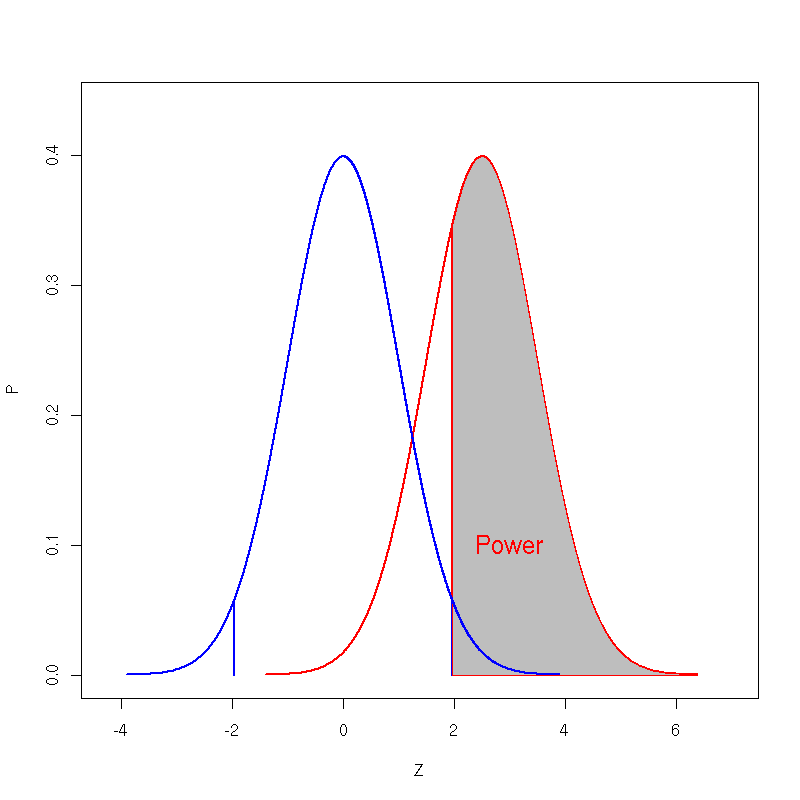
\includegraphics[width=8cm,bb=0 0 800 800]{ZtestBi.png}
    % ZtestBi.png: 800x800 pixel, 72dpi, 28.22x28.22 cm, bb=0 0 800 800
  \end{figure}
\end{frame}

\begin{frame}
  \vspace*{.5cm}
  The \textbf{power} and \textbf{sample size} analysis is an important tool that allows:
  \begin{itemize}
    \vspace*{.75cm}
    \item to check the ability of a statistical test to detect when the null hypothesis is false,
    \vspace*{.75cm}
    \item and to find the needed sample size to reach a specified probability of rejecting the null hypothesis when it is false.
  \end{itemize}
\end{frame}

\begin{frame}
  \vspace*{.25cm}
  In a generic statistical test, when the hypothesis system ($H_0$ against $H_A$) has been set up, the statistical procedure follows these steps:
  \begin{itemize}
    \vspace*{.25cm}
    \item[\checkmark] \textbf{BEFORE} collecting the data (the sample) from the population:
    \begin{enumerate}
    \vspace*{.25cm}
      \item look for a suitable \textbf{statistics}, called \textbf{test statistics}, i.e., a function of data which summarizes specific characteristics of sample and gives information about the hypothesis system. Since the sampling is made randomly, the test statistics value shall be a random value. Also, the test statistics should be chosen so that it ``behave'' in two distinct manners, depending from the actual trueness of $H_0$ or $ H_A $; for example, if $H_0$ is true, then the test statistics value should be ``small'', whereas, if $ H_A $ is true, then the test statistics value should be ``large'';
      \vspace*{.25cm}
      \item evaluate the test statistics \textbf{distribution} when $H_0$ is true;
    \end{enumerate}
  \end{itemize}
\end{frame}

\begin{frame}
  \vspace*{.25cm}
  \begin{itemize}
    \item[] 
    \begin{enumerate}
      \setcounter{enumi}{+2}
      \item determine a \textbf{threshold} value on potential values of test statistics, such that it is able to discriminate between $H_0$ or $ H_A $. Since the test statistics will be a random value, the threshold should be chosen so that the probability of rejecting $H_0$, when it is true, is ``small''. That probability is usually denoted by {\boldmath$\alpha$}.
    \end{enumerate}
  \end{itemize}
  \vspace{1cm}
  \begin{itemize}
    \item[\checkmark] \textbf{AFTER} collecting the data (the sample) from the population:
    \vspace*{.25cm}
    \begin{enumerate}
      \item calcuate the test statistics value based on sample data;
      \vspace*{.25cm}
      \item given this value of test statistics and the threshold value, draw a conclusion about the trueness of $H_0$ or $ H_A $.
    \end{enumerate}
  \end{itemize}
\end{frame}

\begin{frame}
  \begin{small}
    \textbf{PRIOR} to the experiment execution, four conceivable possibility may occur:\\
    \vspace*{.25cm}
    \begin{center}
      \begin{tabular}{|l|c|c|}
        \cline{2-3}
        \multicolumn{1}{c|}{} & The test ``says'' $H_0$ & The test ``says'' $ H_A $ \\
        \hline
        The population ``is'' $H_0$ & OK & \textbf{Type I Error (}{\boldmath$\alpha$}\textbf{)}\\
        \hline
        The population ``is'' $ H_A $ & \textbf{Type II Error (}{\boldmath$\beta$}\textbf{)}   & OK \\
        \hline
      \end{tabular}\\
    \end{center}
    \vspace*{.5cm}
    If the test rejects $H_0$ when $H_0$ is actually true for the population, a \textbf{Type I error} is produced; the probability of this error type is denoted by  {\boldmath$\alpha$}, and it can be controlled by the experimenter.\\
    \vspace*{.25cm}
    If the test accepts $H_0$, when $ H_A $ is the ``true state'' for the studied population, a \textbf{Type II error} is produced; the probability of this error type is denoted by {\boldmath$\beta$}, and it is not directly controllable during the test ``building''. The {\boldmath$(1-\beta)$} value is called test \textbf{power}, and it represents the probability of properly rejecting $H_0$ when it is false.\\
  \end{small}
\end{frame}

\begin{frame}
  \vspace*{.25cm}
  The main parameters resulting from the power analysis are:
  \begin{itemize}
    \item the sample size ({\boldmath $ n $}) or
    \item the test power measure ({\boldmath$1-\beta$})
  \end{itemize}
  and when one of two changes, the other changes accordingly.\\
  \vspace*{.75cm}
  One of two above values can be estimated, for a specific issue, based on existing relationships between 5 quantities:
  \vspace*{.5cm}
  \begin{itemize}
    \item the Type I error \textbf{probability} {\boldmath${\alpha}$}; for this measure the \textbf{``direction'' of \boldmath{$ H_A $} hypothesis} must be specified too: \textbf{one-sided} or \textbf{two-sided};
  \end{itemize}
\end{frame}

\begin{frame}
  \vspace*{.5cm}
  \begin{itemize}
    \item \textbf{the {\boldmath${\beta}$} probability}, i.e., the probability of wrongly reject the alternative hypothesis $ H_A $ (i.e., to accept $H_0$) when it is true;
    \vspace*{.5cm}
    \item the \textbf{{\boldmath${\delta}$} difference} value, between the hypothesized and the true value of the studied quantity (or the difference \textbf{d} between the hypothesized and the true value of test statistics). For example, when considering an hypothesis test on one population mean , ${\delta}$ is the difference between the hypothesized mean $\mu_0$, and the true population mean $\mu$; when considering a test on two independent means, ${\delta}$ is the difference between $\mu_A$ and $\mu_B$;
  \end{itemize}
\end{frame}

\begin{frame}
  \vspace*{.25cm}
  \begin{itemize}
    \item the population \textbf{variance}{ \boldmath $ \sigma^2 $}, if known, or an \textbf{estimate} {\boldmath $ {s^2} $} of population variance, when the \textbf{true variance} {\boldmath$\sigma^2$} \textbf{is unknown};
    \vspace*{.5cm}
    \item \textbf{the sample size {\boldmath $ n $}}, or the sample size of each subgroup of whole sample, if more than only 1 sample shall be considered.
  \end{itemize}
\end{frame}
% ======================================= %



\livelloA{Introduction to logistic regression}

\livelloB{Logistic model}

\begin{frame}
  Suppose we want to predict whether someone is male or female (M=1, F=0) using height in centimeters. We could plot the relations between the two variables as we customarily do in regression. The plot might look something like this:
  \begin{figure}
    \centering
    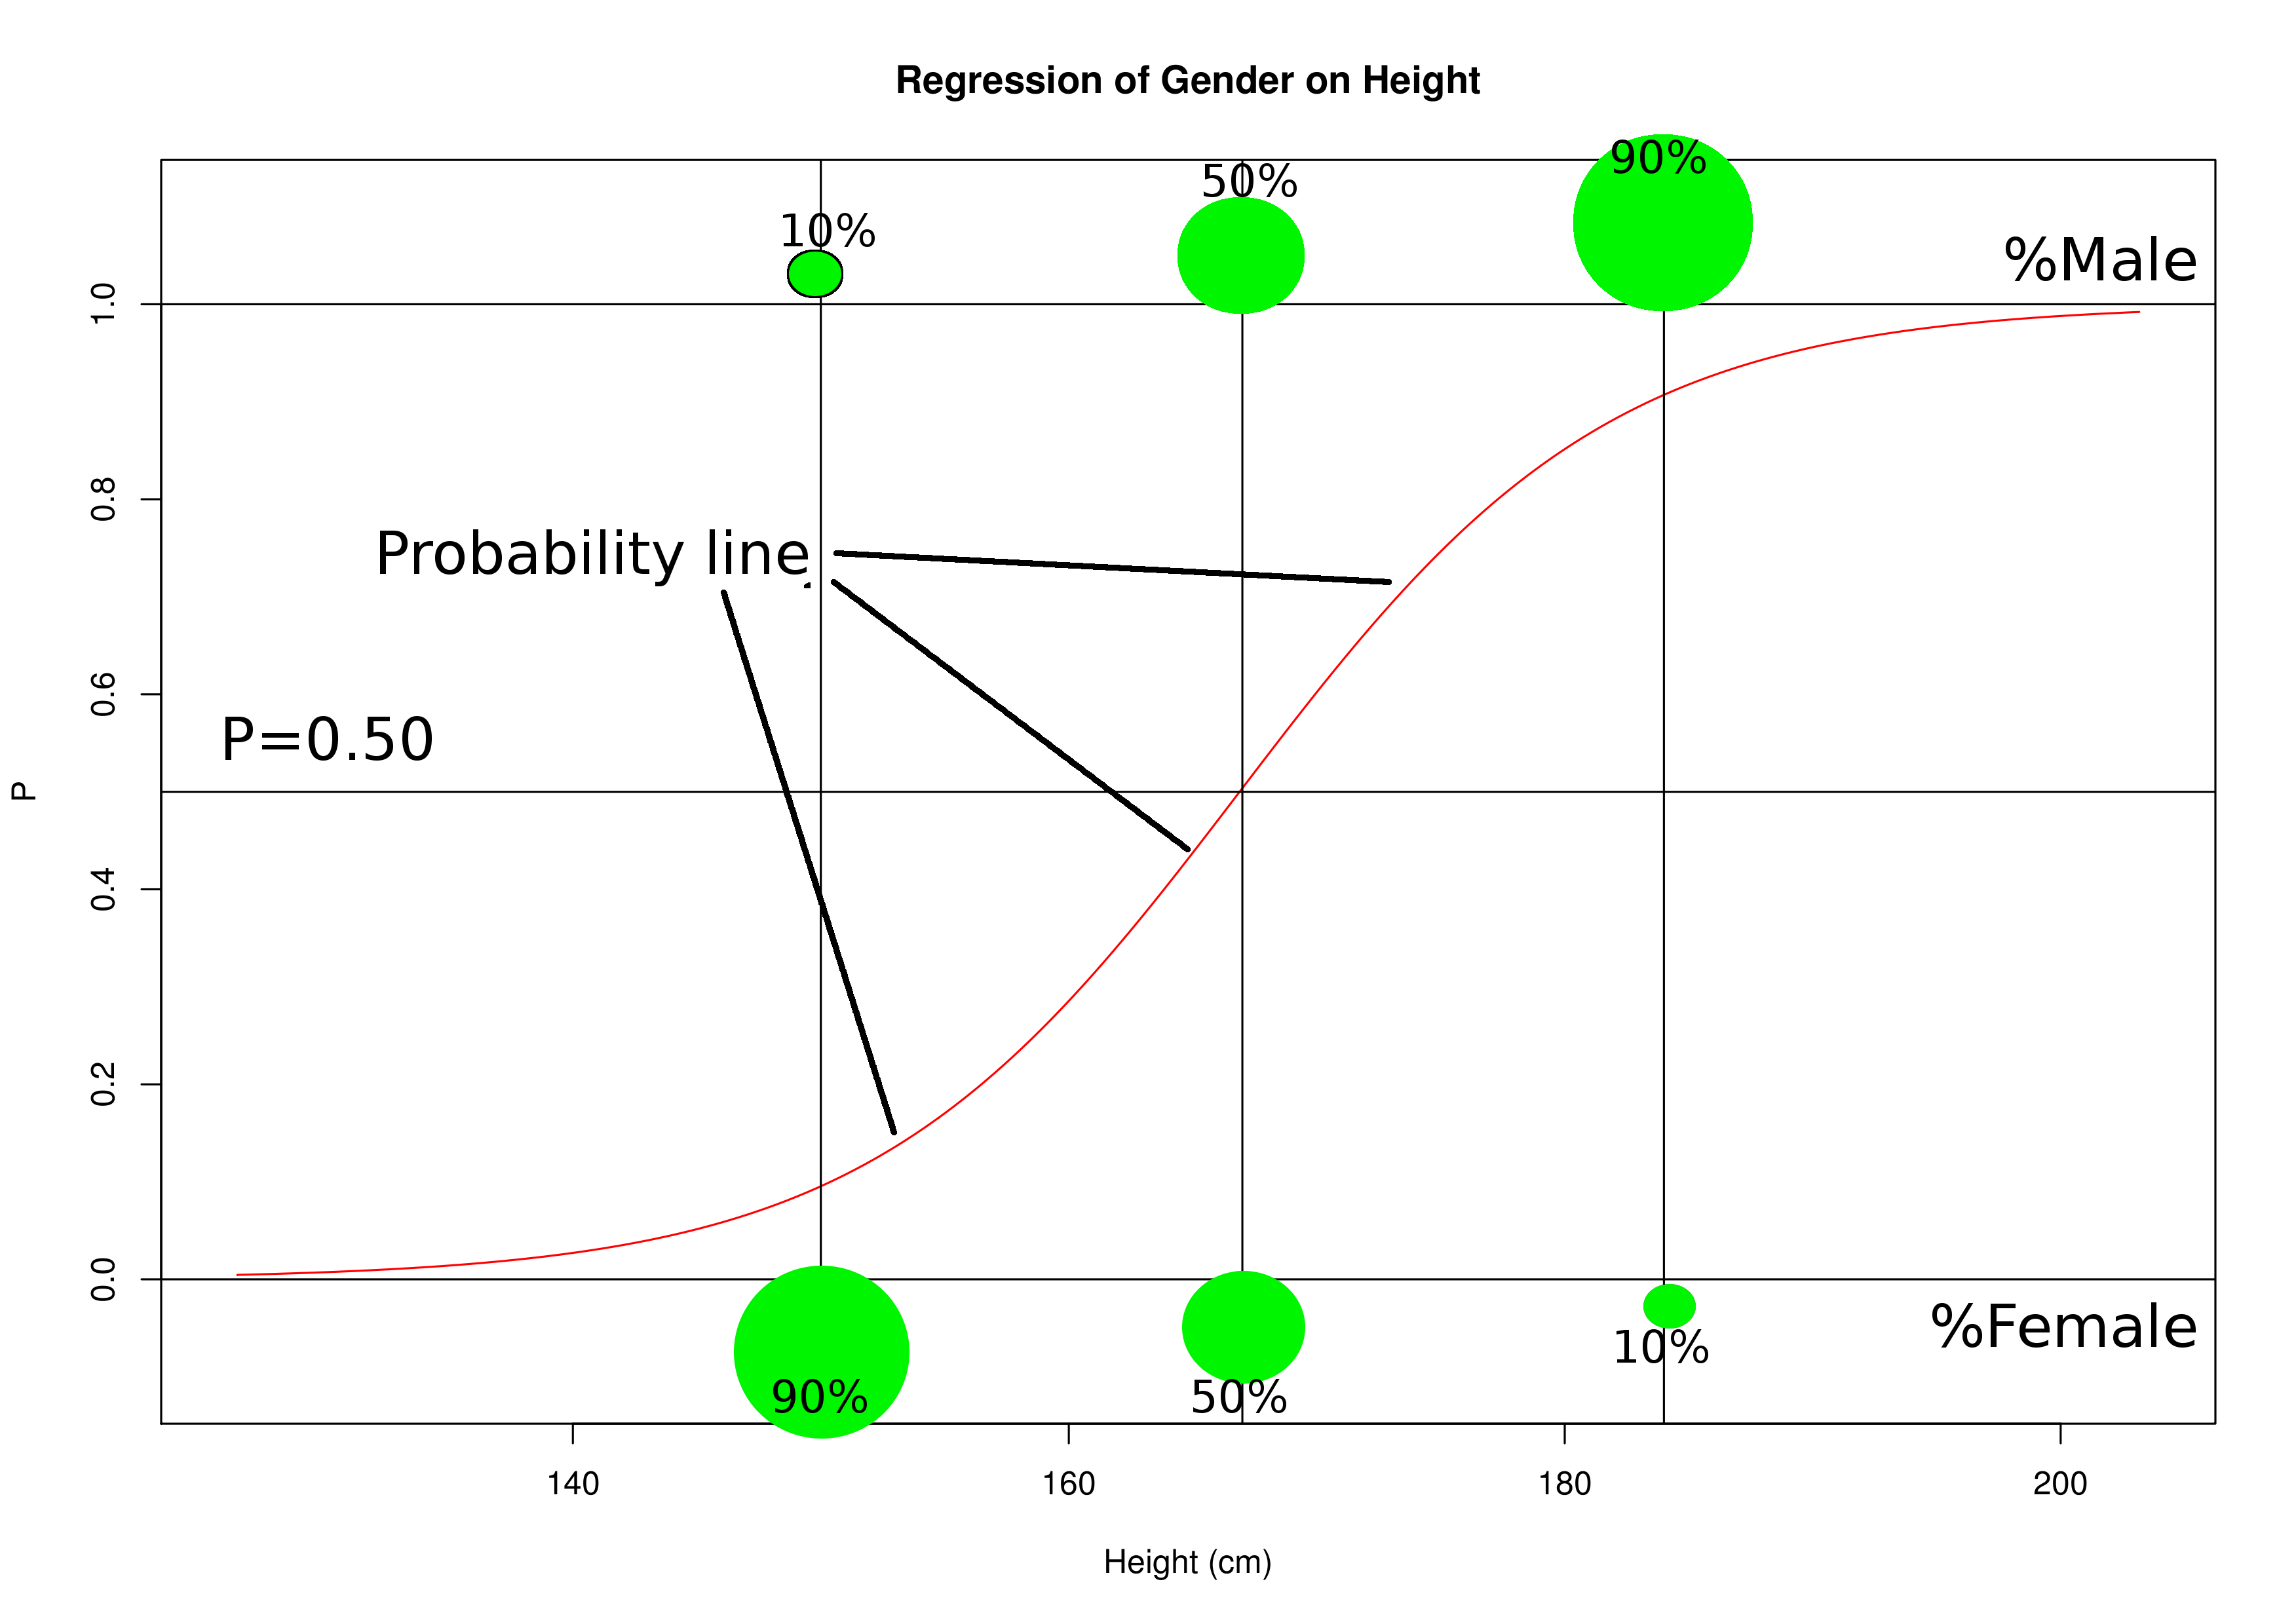
\includegraphics[width=8cm,bb=0 0 841 595]{./../images/logistic.png}
    % logistic.png: 3504x2479 pixel, 300dpi, 29.67x20.99 cm, bb=0 0 841 595
  \end{figure}
\end{frame}

\begin{frame}
  \vspace{.5cm}
  Some points to notice about the graph (data are fictional):
  \begin{itemize}
    \vspace{.35cm}
    \item The regression line is a rolling average, just as in linear regression. The Y-axis is P, which indicates the proportion of 1s at any given value of height. 
    \vspace{.35cm}
    \item The regression line is nonlinear. 
    \vspace{.35cm}
    \item None of the observations --the raw data points-- actually fall on the regression line. They all fall on zero or one. 
  \end{itemize}
\end{frame}

\begin{frame}
 \vspace{.25cm}
  The \textbf{logistic regression} is a ``special type'' of regression where the dependent variable has a Bernoulli($p$) (or a Binomial($n$,$p$)) distribution, and then it can take only $0$ or $1$ values.\\
 \vspace{0.25cm}
  Also, in the logistic regression the main parameter of interest ($p$: the ``success'' probability) must ``fall'' within the $(0,1)$ interval.\\
 \vspace{0.25cm}
  As in ``regular linear'' regression, the logistic regression try to explain the variability of dependent variable based on some independent variables.\\
  \vspace{0.25cm}
  Independent variables, as in linear regression may be quantitative/continuous (as in graph above) as well as qualitative.\\
  \vspace{.25cm}
  (Note: ``multinomial'' and ``ordered multinomial'' types of logistic regression exist too).
\end{frame}

\begin{frame}
 \vspace{.5cm}
  In one of its simplest forms, the mathematical formulation of logistic regression states that the dependent variable ($Y$) has a distribution whose expected value is such that:
 \vspace{0.25cm}
  $$E\{Y\}=p=\dfrac{e^{\alpha+\beta \cdot X}}{1+e^{\alpha+\beta \cdot X}}$$\\
  \vspace{.25cm}
  Where $X$ is the independent variable.\\
  \vspace{.25cm}
  Since the expected value for a Bernoulli variable is $p$ (the probability of ``success''), the above formula states that the success probability is linked to the $X$ independent variable by a logistic relation or, equivalently, that\\
  $$ln\left(\dfrac{p}{1-p}\right)=\alpha+\beta \cdot X$$
\end{frame}

\livelloB{Logistic model estimates}

\begin{frame}
  \vspace{.5cm}
  The estimation of logistic model is a complex mathematical/statistical matter.\\
  \vspace{.5cm}
  Usually, the more reliable method is the Maximum Likelihood estimation.\\
  \vspace{.5cm}
  This method allows to estimate all the parameters included in model (remember that the model illustrated above is one of simplest models), with error and significancy evaluation too.\\
  \vspace{.5cm}
  The exponential of estimated parameters, anyway, are estimates of odds-ratio for the specific effect involved by the parameter itself.
\end{frame}

\begin{frame}
 \vspace{.25cm}
 \textbf{Example:}\\
  \vspace{.25cm}
  A sample of 40 height readings has been collected: 20 males and 20 females. The data are the following:\\
  \begin{tiny}
    \begin{center}
      \begin{tabular}{l|r r r r r r r r }
        gender & F & F & F & F & F & F & F & F \\
        height & 158.2512 & 168.455 & 157.8914 & 164.0353 & 164.0082 & 147.6034 & 141.7605 & 155.4557\\
        \hline
        gender & F & F & F & F & F & F & F & F \\
        height & 165.6356 & 174.7999 & 165.8107 & 151.6972 & 174.2301 & 161.6354 & 177.6935 & 154.0353\\
        \hline
        gender & F & F & F & F & M & M & M & M \\
        height & 175.0083 & 160.0799 & 169.4225 & 183.6644 & 165.6596 & 185.3086 & 175.7386 & 168.63 \\
        \hline
        gender & M & M & M & M & M & M & M & M \\
        height & 170.4932 & 179.8414 & 163.6995 & 148.1559 & 183.6873 & 169.3332 & 179.484 & 175.2373\\
        \hline
        gender & M & M & M & M & M & M & M & M \\
        height & 164.1659 & 172.8038 & 182.1371 & 160.7205 & 185.0418 & 169.9699 & 170.6346 & 166.1434\\
      \end{tabular}
    \end{center}
  \end{tiny}
\end{frame}

\begin{frame}
  \vspace{.25cm}
  Estimating the probability of being ``Male'' via logistic model, gives the results:\\
  \begin{center}
    \begin{tabular}{lrrrr}
      Coefficients: &&&&\\
      \hline
      & Estimate & Std. Error &z value & Pr($>|z|$) \\
      \hline
      (Intercept) & -14.45785 & 6.31375  & -2.290  & 0.0220 \\
      height       & 0.08612   & 0.03750  & 2.297   & 0.0216 \\
      \hline
    \end{tabular}
  \end{center}
  The table shows that the probability of having a Male is given by:
  $$Pr\{Y=``Male''\}=\dfrac{e^{-14.45785+0.08612 \cdot height}}{1+e^{-14.45785+0.08612 \cdot height}}$$\\
  Note: the positive estimated coefficient for the \texttt{height} variable means that the probability of having a Male ``grows'' with the height of subject.
\end{frame}

\begin{frame}
  \begin{figure}
    \centering
    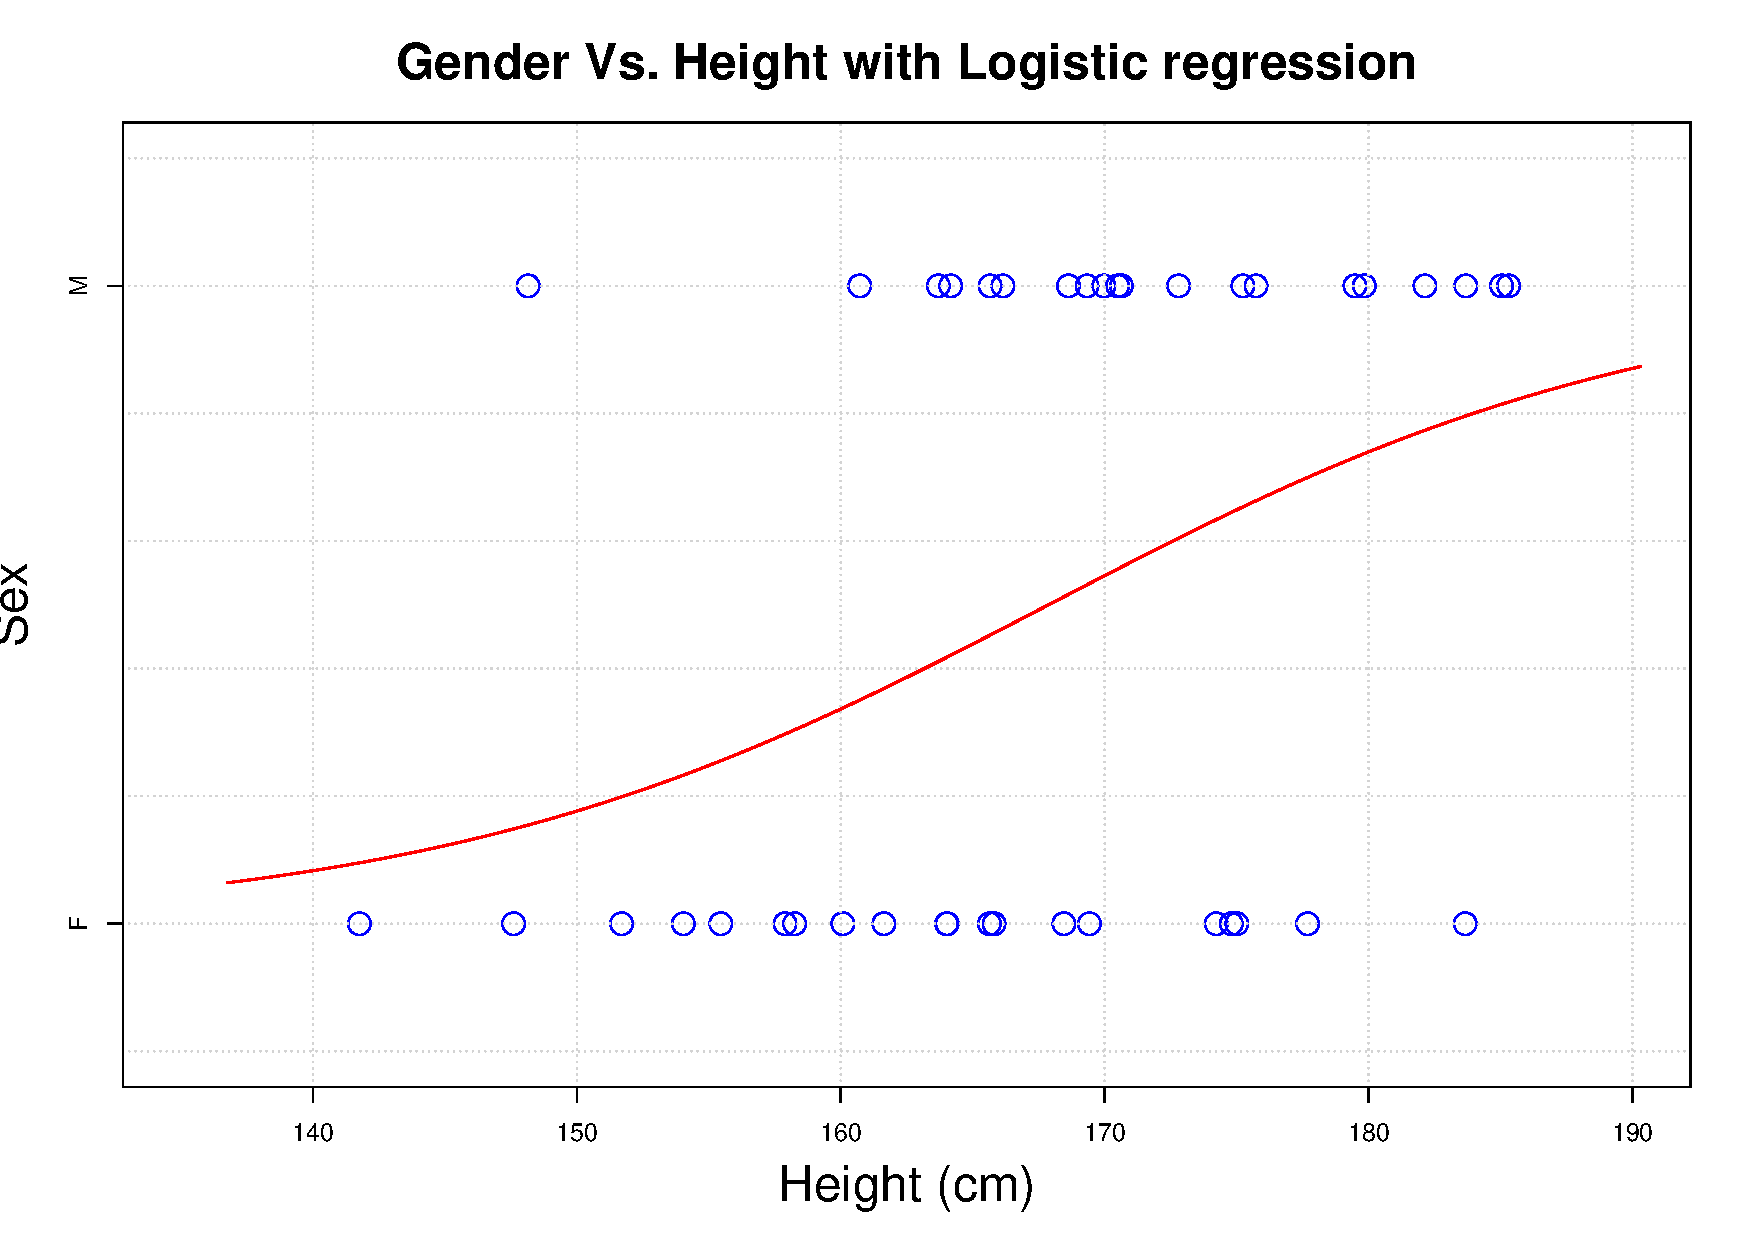
\includegraphics[width=10cm]{logisticEst.pdf}
    % logisticEst.png: 3504x2479 pixel, 300dpi, 29.67x20.99 cm, bb=
  \end{figure}
\end{frame}

\livelloB{Odds, logit, odds-ratio}
\begin{frame}
  \vspace{.25cm}
  In above slides, some new quantities were used. The quantity:\\
  $$\dfrac{p}{1-p}$$\\
  is called \textbf{Odds}.\\
  \vspace{.75cm}
  The quantity\\
  $$ln\left(\dfrac{p}{1-p}\right)$$\\
  is called \textbf{Logit}.
\end{frame}

\begin{frame}
  \vspace{.25cm}
  Note that, for example, in above case of Male/Female distinction, odds can also be found by counting the number of people in each group and dividing one number by the other. \\
  \vspace{.5cm}
  The probability is not the odds. \\
  \vspace{.5cm}
  In example, the odds of being male would be .90/.10 or 9 to one, and the odds of being female would be .10/.90 or 1/9 or .11. This asymmetry is unappealing.\\
  \vspace{.5cm}
  The natural log of odds makes the logit values symmetrical around 0 (zero).\\
\end{frame}

\begin{frame}
  \vspace{.25cm}
  In a simpler ``two groups'' example, where male and female subjects should be predicted using only one qualitative variable with only two categories (e.g., foot size: Small or Big), the \textbf{odds-ratio} $\mathbf{\phi}$ may be used to show ``how much the independent variable is able to predict the dependent variable''.\\
  Suppose that the relationship between Gender and Foot size can be expressed in this form:
  \begin{center}
    \begin{tabular}{l|c|c}
      & Big & Small\\
      \hline
      Male & $a$ & $b$\\
      \hline
      Female & $c$ & $d$
    \end{tabular}
  \end{center}
  In this case, the odds-ratio is:\\
  $$\phi=\text{odds-ratio}=\dfrac{\frac{a}{a+c}/\frac{c}{a+c}}{\frac{b}{b+d}/\frac{d}{b+d}}=\dfrac{a d}{b c}$$
\end{frame}

\begin{frame}
  \vspace{.25cm}
  Odds-ratio express the multiplicative change in probability rate between Male and Female subject when changing (in this case) the foot size from Small to Big.
  In above example, suppose that the table contains these data:
  \begin{center}
    \begin{tabular}{l|c|c}
      & Big & Small\\
      \hline
      Male & 80 & 15\\
      \hline
      Female & 10 & 90
    \end{tabular}
  \end{center}
  Here, the Male Vs Female odds-ratio is $48$.\\
  \vspace{.25cm}
  That means that the relative probability of having a Male subject with respect to having a Female subject from Small foot to Big foot, grows 48 times.
\end{frame}

\begin{frame}
  \vspace{.25cm}
  \textbf{Example:}\\
  \vspace{.25cm}
  If the above table is used to estimate the probability of being ``Male'' via logistic model, the model estimate result is:\\
  \begin{center}
    \begin{tabular}{lrrrr}
      Coefficients: &&&&\\
      \hline
      & Estimate & Std. Error &z value & Pr($>|z|$) \\
      \hline
      (Intercept)  & 2.0794  &  0.3354  & 6.200 & 5.65e-10 \\
      foot:Small  & -3.8712   & 0.4362  & -8.875  & $<$ 2e-16 \\
      \hline
    \end{tabular}
  \end{center}
  The table show that the probability of having a Male is given by:
  $$Pr\{Y=``Male''\}=\dfrac{e^{2.0794-3.8712 \cdot foot}}{1+e^{2.0794-3.8712 \cdot foot}}$$\\
  Where foot=0 means ``Big foot'', and foot=1 means ``Small foot''
\end{frame}

\begin{frame}
  \vspace{.25cm}
  The second line of table contents, show that the probability of having a Male changing the foot size from Big to Small reduces such that the $log(\text{odds-ratio})=-3.8712$.\\
  \vspace{1cm}
  Consequently, the odds-ratio of change from Big to Small foot is\\
  $$\phi=e^{-3.8712}\simeq 0.02083335$$
  \vspace{.5cm}
  very close to 1/48=0.0208333333 obtained from above calculations.
\end{frame}
% ======================================= %



\livelloA{Appendix: Continuous distributions}

\livelloB{Normal}

\begin{frame}
  \vspace{.25cm}
  For theoretical reasons (such as the central limit theorem), any variable that is the sum of a large number of independent factors is likely to be normally distributed. For this reason, the normal distribution is widely used in statistics, natural science, and social science as a simple model for complex phenomena. \\
  \vspace{.75cm}
  For example, the error in an experiment is usually assumed to follow a normal distribution, and the propagation of uncertainty is computed using this assumption.
\end{frame}

\begin{frame} 
  \vspace*{.25cm}
  The normal distribution ($N(\mu,\sigma)$) is defined by two parameters:
  \begin{itemize}
    \item $\mu$, determines the position of the distribution;
    \item $\sigma$, determines the ``variability'' or ``dispersion'' of the distribution.
  \end{itemize}
  \vspace*{.75cm}
  The normal distribution is defined between $-\infty$ and $+\infty$, and, being a probability distribution, his integral from $-\infty$ to $+\infty$ is equal to 1.\\
  \vspace*{.75cm}
  Asymptotically tends to zero, and  the tails over the value $6\sigma$, with good approximation, can be considered truncated.\\
\end{frame}

\begin{frame}
  \vspace{-0.25cm}
  \begin{center}
    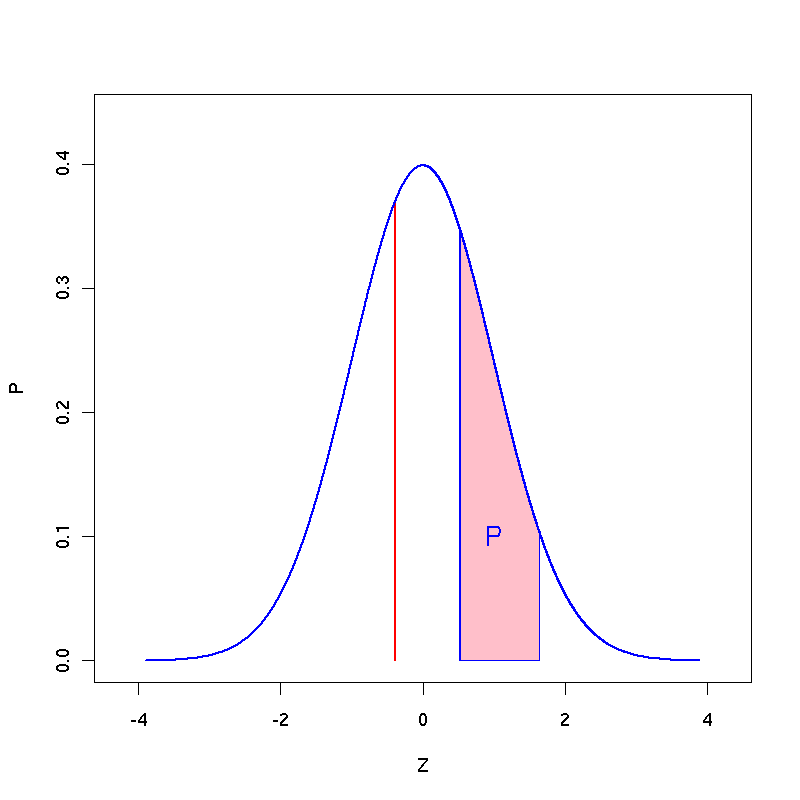
\includegraphics[scale=0.3]{g2.png}
  \end{center}
\end{frame}

\begin{frame} 
  \vspace*{.15cm}
  The mathematical formulation for the normal distribution is:
  \vspace*{.15cm}
  $$y=f(x)=\frac{1}{\sigma \sqrt{2\pi}}\, e^{-\frac{1}{2}\left ( \frac{x-\mu}{\sigma}\right)^2}.$$  \\
  \vspace*{.15cm}
  This is the expression of \textbf{probability density function (pdf)} of normal distribution.\\
  \vspace*{.15cm}
  \textbf{It allows to evaluate the value of Y (ordinate value) for all X values (abscissa value)}.\\
  \vspace*{.15cm}
  The $\mu$ and $\sigma$  values define totally the probability density function.\\
  \vspace*{.15cm}
  \textbf{The density normal curves are infinite}.\\
  \vspace*{.15cm}
  When $\mu=0$ and $\sigma=1$, then the Normal distribution is said a \textbf{standard normal distribution}.
\end{frame}

\begin{frame} 
  \vspace*{.25cm}
  Graph for  a Normal Distribution.\\
  \vspace*{.25cm}
  \begin{figure}
    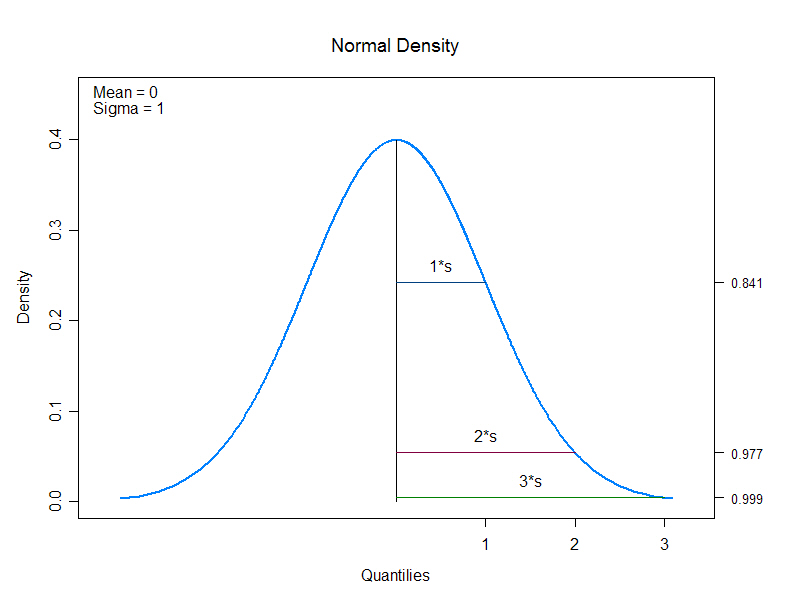
\includegraphics[scale=0.3]{2_25.png}
  \end{figure}
\end{frame}

\begin{frame} 
  \vspace*{.25cm}
  If {\boldmath$\mu $} changes and {\boldmath$\sigma$} is constant, there are infinite normal curves with the same  shape and size, but with a different axis of symmetry.
  \begin{figure}
    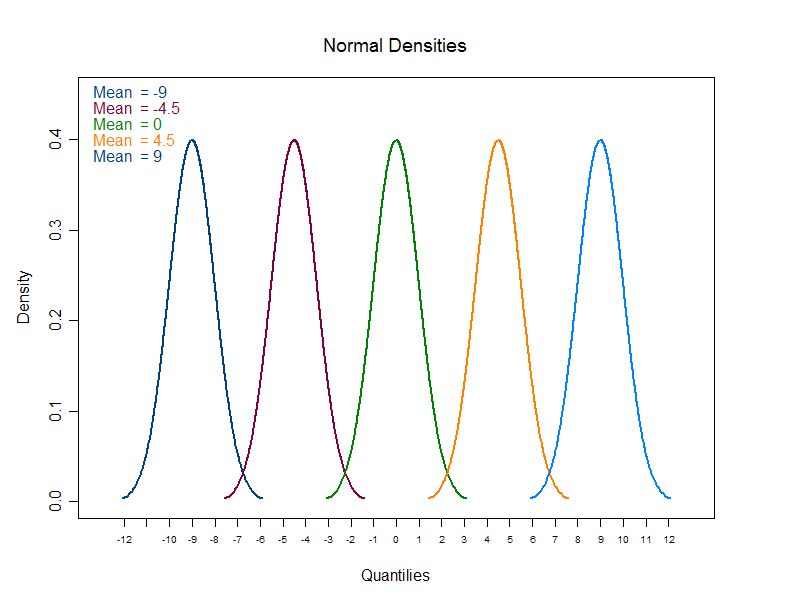
\includegraphics[scale=0.3]{2_27.png}
  \end{figure}
\end{frame}

\begin{frame} 
  \vspace*{.25cm}
  If {\boldmath$\mu $} is constant and  {\boldmath$\sigma$} changes, all the infinite curves have the same symmetry axis, but {\boldmath$\sigma$} determines their shape.
  \begin{figure}
    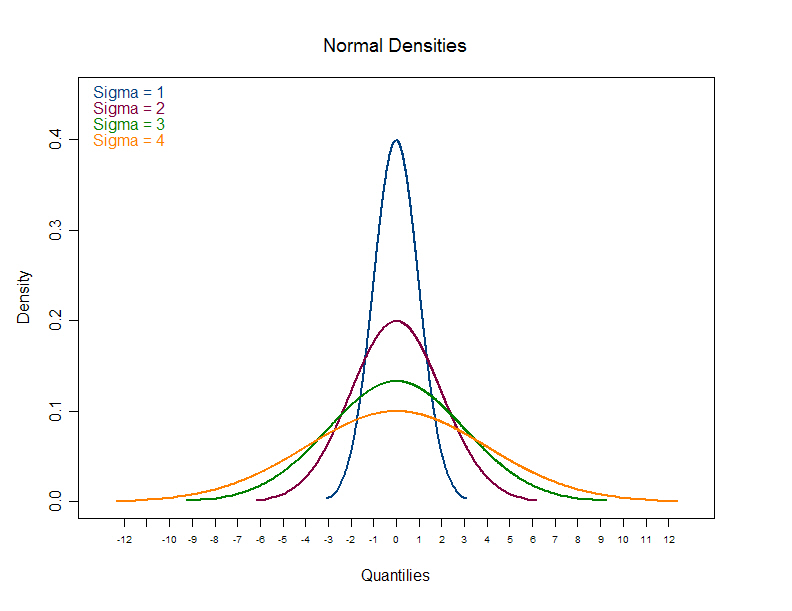
\includegraphics[scale=0.3]{2_28.png}
  \end{figure}
\end{frame}

\begin{frame} 
  \vspace*{.25cm}
  In this case both {\boldmath$\mu $} and {\boldmath$\sigma$} are different:\\
  \begin{figure}
    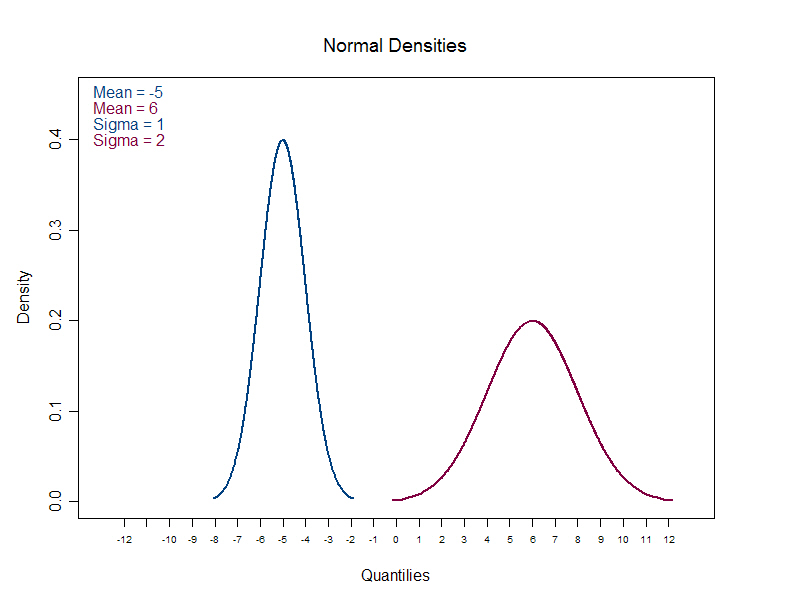
\includegraphics[scale=0.3]{2_29.png}
  \end{figure}
\end{frame}

\begin{frame} 
  \vspace*{.25cm}
  This graph shows some relevant probabilities for the Normal distribution:\\
  \begin{figure}
    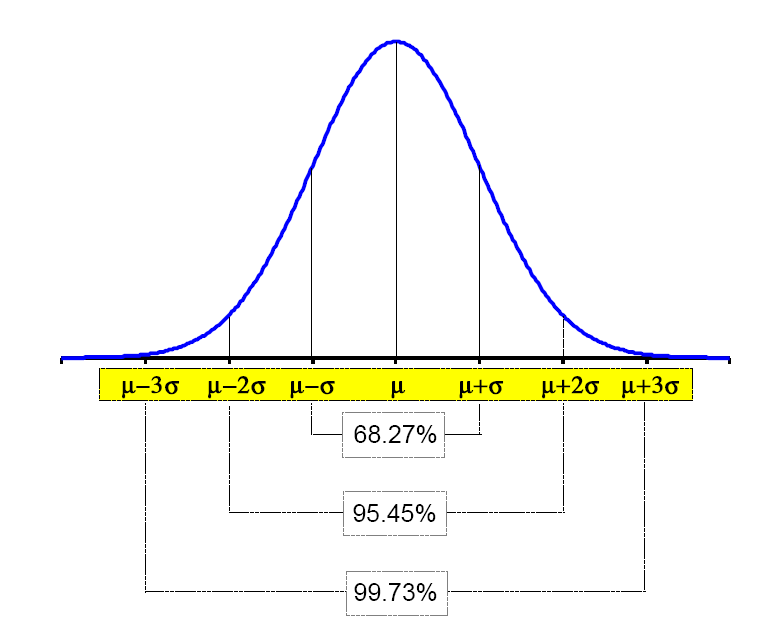
\includegraphics[scale=0.3]{2_34.png}
  \end{figure}
\end{frame}

\livelloB[Chi-square ($\chi^2_\nu$)]{Chi-square}

\begin{frame}
  \vspace*{1cm}
  The {\boldmath $ \chi_\nu^2 $} random variable is a random variable obtained by summing up the square of $ \nu $ independent standard normals ($ \mu = 0 $ and $ \sigma = 1 $) $ Z_1,\;  Z_2,\;  \dots,\; Z_\nu $:\\
  $$\chi^2_\nu=Z_1^2 + Z_2^2 + \dots + Z_\nu^2$$\\
  \vspace*{.75cm}
  The $ \chi^2 $ probability density function (pdf) is determined \textbf{by only {\boldmath $ \nu $} parameter}, i.e., the number of degrees of freedom ($df$).\\
\end{frame}

\begin{frame}
  \vspace*{.5cm}
  The pdf is defined between $ 0 $ and $ +\infty $:\\
  \vspace{.5cm}
  $$y=f(x)=\dfrac{1}{2^{\frac{\nu}{2}} \Gamma(\nu/2)} x^{\frac{\nu}{2}-1} e^{-\frac{x}{2}}$$\\
  \vspace{.5cm}
  Where $\Gamma(\cdot)$ is the Gamma function.\\
  \vspace{1cm}
  When $\nu$ grows, the pdf tends to be similar to a Normal distribution.
\end{frame}

\begin{frame}
  \vspace*{.5cm}
  \centering
  The next graph shows the $ \chi^2_{df} $ distribution for several $ df $ values.\\
  \begin{figure}
    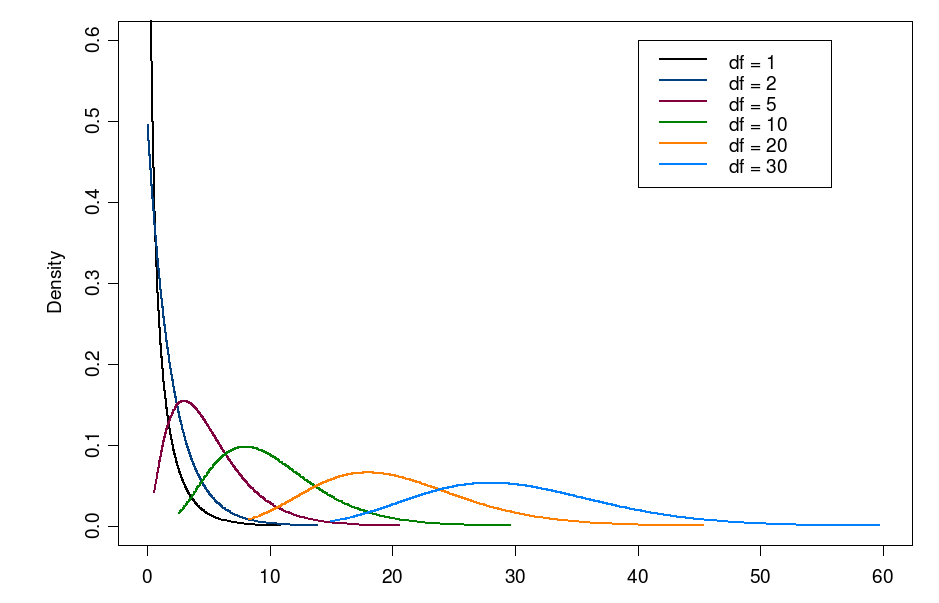
\includegraphics[scale=0.33]{2_37.png}
  \end{figure}
\end{frame}





\end{document}
